% ==========================================
% Step 4/4 - Final refinement (refinement step 3)
% Output: step4-02-19-2026-thursday-week1-Analysis_II-_mehrere_Variablen-offset-final.tex
% Input: step3-02-19-2026-thursday-week1-Analysis_II-_mehrere_Variablen-offset-speech_refined.tex
% Model: gemini-3.7-flash
% Temperature: 0.35
% TopP: 0.9
% TopK: 10
% MaxOutputTokens: 65535
% ThinkingBudget: 4096
% ThinkingLevel: MEDIUM
% Processed on: 2026-10-12 20:55:05
% ------------------------------------------
% Token Usage (1 Request(s)):
%   - Total Prompt Tokens : 66'006 (gesamter Prompt, inkl. Cache)
%   - Cached Context      : 0 (aus Google Context-Cache, rabattiert)
%   - Fresh Input Tokens  : 66'006 (neu verrechneter Input)
%   - Output Tokens       : 33'852 (generiertes LaTeX, ohne Thinking)
%   - Thinking Tokens     : 15'601 (Denk-Tokens, als Output verrechnet)
% ==========================================
% ==========================================
% Step 3/4 - Speech refinement (refinement step 2)
% Output: step3-02-19-2026-thursday-week1-Analysis_II-_mehrere_Variablen-offset-speech_refined.tex
% Input: step2-02-19-2026-thursday-week1-Analysis_II-_mehrere_Variablen-offset-merged.tex
% Model: gemini-3.7-flash
% Temperature: 0.35
% TopP: 0.9
% TopK: 10
% MaxOutputTokens: 65535
% ThinkingBudget: 4096
% ThinkingLevel: MEDIUM
% Processed on: 2026-10-12 20:48:22
% ------------------------------------------
% Token Usage (1 Request(s)):
%   - Total Prompt Tokens : 230'263 (gesamter Prompt, inkl. Cache)
%   - Cached Context      : 228'464 (aus Google Context-Cache, rabattiert)
%   - Fresh Input Tokens  : 1'799 (neu verrechneter Input)
%   - Output Tokens       : 33'112 (generiertes LaTeX, ohne Thinking)
%   - Thinking Tokens     : 32'395 (Denk-Tokens, als Output verrechnet)
% ==========================================
% ==========================================
% Step 2/4 - Merge & timestamp alignment (refinement step 1)
% Output: step2-02-19-2026-thursday-week1-Analysis_II-_mehrere_Variablen-offset-merged.tex
% Input: step1-02-19-2026-thursday-week1-Analysis_II-_mehrere_Variablen-all-offset.tex
% Model: gemini-3.7-flash
% Temperature: 0.4
% TopP: 0.95
% TopK: 40
% MaxOutputTokens: 65535
% ThinkingBudget: 32765
% ThinkingLevel: MEDIUM
% Processed on: 2026-10-12 20:31:28
% ------------------------------------------
% Token Usage (1 Request(s)):
%   - Total Prompt Tokens : 204'037 (gesamter Prompt, inkl. Cache)
%   - Cached Context      : 0 (aus Google Context-Cache, rabattiert)
%   - Fresh Input Tokens  : 204'037 (neu verrechneter Input)
%   - Output Tokens       : 42'933 (generiertes LaTeX, ohne Thinking)
%   - Thinking Tokens     : 11'002 (Denk-Tokens, als Output verrechnet)
% ==========================================
% ==========================================
% Step 1/4 - Transcription, 4 part(s) combined
% Output: step1-02-19-2026-thursday-week1-Analysis_II-_mehrere_Variablen-all-offset.tex
% Source video: 02-19-2026-thursday-week1-Analysis_II-_mehrere_Variablen-speed-1-compressed.mp4
% Model: gemini-3.7-flash
% Temperature: 0.36
% TopP: 0.95
% TopK: 40
% MaxOutputTokens: 65535
% ThinkingBudget: 32765
% ThinkingLevel: HIGH
% Processed on: 2026-10-12 20:17:42
% ------------------------------------------
% Parts:
%   - Part 1: 02-19-2026-thursday-week1-Analysis_II-_mehrere_Variablen-part1.mp4 | start 00:00:00 | model gemini-3.7-flash | processed 2026-10-12 19:49:46 | prompt 337'889 | output 13'342 | thinking 18'979
%   - Part 2: 02-19-2026-thursday-week1-Analysis_II-_mehrere_Variablen-part2.mp4 | start 00:19:59 | model gemini-3.7-flash | processed 2026-10-12 19:57:03 | prompt 350'143 | output 12'251 | thinking 24'474
%   - Part 3: 02-19-2026-thursday-week1-Analysis_II-_mehrere_Variablen-part3.mp4 | start 00:39:58 | model gemini-3.7-flash | processed 2026-10-12 20:07:59 | prompt 361'432 | output 12'929 | thinking 23'245
%   - Part 4: 02-19-2026-thursday-week1-Analysis_II-_mehrere_Variablen-part4.mp4 | start 00:59:57 | model gemini-3.7-flash | processed 2026-10-12 20:17:41 | prompt 373'345 | output 12'030 | thinking 26'956
% ------------------------------------------
% Token Usage of this run (4 Request(s)):
%   - Total Prompt Tokens : 1'422'809 (gesamter Prompt, inkl. Cache)
%   - Cached Context      : 0 (aus Google Context-Cache, rabattiert)
%   - Fresh Input Tokens  : 1'422'809 (neu verrechneter Input)
%   - Output Tokens       : 50'552 (generiertes LaTeX, ohne Thinking)
%   - Thinking Tokens     : 93'654 (Denk-Tokens, als Output verrechnet)
% ==========================================

% Primary Language: English
% End of the video: 01:23:55

\lecturechapter[1]{Thursday}{19 Feb}{19 February 2026}{Open and Closed Sets, Topology, and Continuity in Metric Spaces}

\begin{overview}[Course Content Overview: Topology and Continuity in Metric Spaces]
In this lecture, we transition from sequential notions in metric spaces (convergence, Cauchy sequences, and completeness) to the topological foundations of multi-variable analysis:
\begin{itemize}
    \item \textbf{Open Balls and Open Sets:} Defining open balls $B(x, r)$ and open subsets $U \subseteq X$ via local ball containment.
    \item \textbf{Closed Sets and Topology:} Defining closed sets via complements and introducing the metric topology $\mathcal{T}$ associated to a distance $d$.
    \item \textbf{Stability Properties:} Proving that arbitrary unions and finite intersections of open sets are open, and employing De Morgan's laws to establish dual properties for closed sets.
    \item \textbf{Interior, Closure, and Boundary:} Formalizing $\operatorname{int}(\Omega)$, $\overline{\Omega}$, and $\partial\Omega$, with concrete geometric examples in Euclidean space $\mathbb{R}^2$.
    \item \textbf{Sequential Characterization:} Characterizing openness and closedness via convergent sequences and the concept of eventual containment.
    \item \textbf{Continuity in Metric Spaces:} Formulating the three equivalent characterizations of continuity ($\varepsilon$-$\delta$, sequential, and topological pre-images of open sets).
\end{itemize}
\end{overview}

\section{Review of Metric Spaces and Motivation}

\begin{speech}[00:00:00 - 00:01:50]
Good afternoon. We can continue where we left off last time.

Just a quick summary of what we saw in the last lectures: The first lecture was mostly an introduction, but then we saw metric spaces. And I told you --- because people already asked me, even though I addressed it the first day --- why we study metric spaces. Whenever it gets too abstract, the model you need to have in mind all the time for this $(X, d)$ metric space is $\mathbb{R}^n$ with the Euclidean distance, okay? So, whenever you have doubts, just plug $\mathbb{R}^n$ where there is an $X$ --- a capital $X$ --- and $d$ is the usual distance, the modulus of the difference of the points.

And I said that I wanted to do this in this more general framework because later, in the last part of the course, we will use other spaces, okay? And for good reason: we will use the space of continuous functions to prove some theorems in the course. But if you want --- this is not something that belongs only to mathematicians, right? Let me say very quickly for the physicists: in classical mechanics, the point in space is a vector in $\mathbb{R}^n$, right? But when you go to quantum mechanics, what is a point? What is the position of a particle in space? It's the wave function; it's a function. So, the wave functions are naturally points in your space, right?

This is what we are saying here: We are trying to state things more generally to be able to understand the things that come naturally in physics, for instance.
\end{speech}

\begin{speech}[00:01:50 - 00:02:24]
Okay. Now, in this framework of metric spaces, we saw what a sequence means, what it means that a sequence converges, what a Cauchy sequence is, and what a complete metric space is. And we proved that $\mathbb{R}^n$ is always a complete metric space, using the fact that $\mathbb{R}$ is complete, last time.

And today we will see the definition of open and closed sets in a metric space, and the notion of continuous functions in the setup of metric spaces. So, let me start with the definition of...
\end{speech}

\begin{content}[Summary of Previous Lectures and Canonical Models]
\textbf{Foundational Concepts in Metric Spaces $(X, d)$:}
\begin{itemize}
    \item \textbf{Canonical Finite-Dimensional Model:} The primary intuitive model for any metric space $(X, d)$ is Euclidean space $\mathbb{R}^n$ equipped with the standard Euclidean distance:
    \[
    d_{\text{Euc}}(x, y) := \|x - y\|_2 = \sqrt{\sum_{i=1}^n (x_i - y_i)^2}.
    \]
    \item \textbf{Sequences and Convergence:} A sequence $(x_n)_{n \ge 0} \subseteq X$ converges to a limit $x \in X$ (written $x_n \to x$) if:
    \[
    \lim_{n \to \infty} d(x_n, x) = 0 \iff \forall \varepsilon > 0 \ \exists N \in \mathbb{N} \ \forall n \ge N \colon d(x_n, x) < \varepsilon.
    \]
    \item \textbf{Cauchy Sequences and Completeness:} A sequence $(x_n)_{n \ge 0}$ is a \newterm{Cauchy sequence} if $\lim_{n, m \to \infty} d(x_n, x_m) = 0$. A metric space $(X, d)$ is \newterm{complete} if every Cauchy sequence in $X$ converges to a limit in $X$. In particular, $(\mathbb{R}^n, d_{\text{Euc}})$ is complete.
\end{itemize}

\begin{steps}[Physical Motivation: From Classical Points to Function Spaces]
In classical mechanics, the state of a point particle is described by a position vector $x \in \mathbb{R}^3$. In quantum mechanics, however, the state of a particle is given by a complex-valued wave function $\psi \colon \mathbb{R}^3 \to \mathbb{C}$ living in an infinite-dimensional function space (such as $L^2(\mathbb{R}^3)$). Developing analysis in general metric spaces allows us to treat such function spaces rigorously using the exact same geometric intuition as $\mathbb{R}^n$.
\end{steps}
\end{content}

\section{Open Balls and Open Sets}

\subsection{Open Balls}

\begin{speech}[00:02:24 - 00:03:54]
...definition of open set... So, let me start maybe with the definition of an open ball. Open ball. \inlinemetanote{writes \qt{defn (open ball)}}

We define the open ball of radius $r$ positive, \inlinemetanote{writes \qt{Define open ball of radius $r > 0$}} centered at a given point $x$ in my metric space, \inlinemetanote{writes \qt{centered at $x \in X$ as}} as --- and we will denote it by this: the ball centered at $x$ with radius $r$ \inlinemetanote{writes $B(x, r)$}; sometimes you will see the equivalent notation of the ball of radius $r$ centered at $x$ \inlinemetanote{writes $B_r(x) = B(x, r)$}, which is also in many notes and books, it's the same, okay? --- this is by definition the set of points in my space such that the distance... Ah, sorry, the points will be $y$, such that the distance between $y$ and $x$ is less than $r$, right? \inlinemetanote{writes $= \{y \in X \mid d(y, x) < r\}$}
\end{speech}

\begin{content}
\begin{definition}[Open Ball]\label[definition]{def:open-ball}
Let $(X, d)$ be a metric space. For any point $x \in X$ and any real number $r > 0$, the \newterm{open ball} of radius $r$ centered at $x$ is defined as the set:
\begin{equation}\label{eq:open-ball-def}
B(x, r) := \{ y \in X \mid d(y, x) < r \}.
\end{equation}
\end{definition}

\begin{notation}[Alternative Notation for Open Balls]\label[notation]{not:open-ball}
In mathematical literature and lecture notes, the open ball is frequently denoted by $B_r(x)$ interchangeably with $B(x, r)$:
\[
B_r(x) \equiv B(x, r).
\]
\end{notation}

\begin{steps}[Key Structural Features of Open Balls]
\begin{itemize}
    \item \textbf{Strict Inequality:} The condition defining the ball is strictly $d(y, x) < r$, excluding points at distance exactly equal to $r$.
    \item \textbf{Symmetry:} Since any metric satisfies $d(y, x) = d(x, y)$, the definition can equivalently be written as $d(x, y) < r$.
    \item \textbf{Center Inclusion:} Since $d(x, x) = 0 < r$ for any $r > 0$, the center point $x$ is always an element of $B(x, r)$.
\end{itemize}
\end{steps}
\end{content}

\begin{speech}[00:03:54 - 00:04:52]
So, if you want a drawing of that, in Euclidean space --- in a general metric space I cannot draw anything because it's too general, but in Euclidean space, let's say in $\mathbb{R}^2$ \inlinemetanote{writes $\mathbb{R}^2$} --- the metric ball would be the ball.

The open ball would be this, right? \inlinemetanote{draws open disk with center $x$, radius $r$, and dashed boundary} What is inside of the ball. And it's open because you don't include... If you want, I can put the boundary of the ball, which we will introduce today also in a general topological space, what the boundary means. This surface of the ball is not included, because there is a strict inequality, okay?

The points that are at distance exactly $r$, I don't take them. This is the open ball.
\end{speech}

\begin{content}[Geometric Representation of an Open Ball in \texorpdfstring{$\mathbb{R}^2$}{R2}]
In the Euclidean plane $(\mathbb{R}^2, d_{\text{Euc}})$, an open ball $B(x, r)$ corresponds geometrically to an open circular disk whose boundary circle is excluded.

\begin{center}
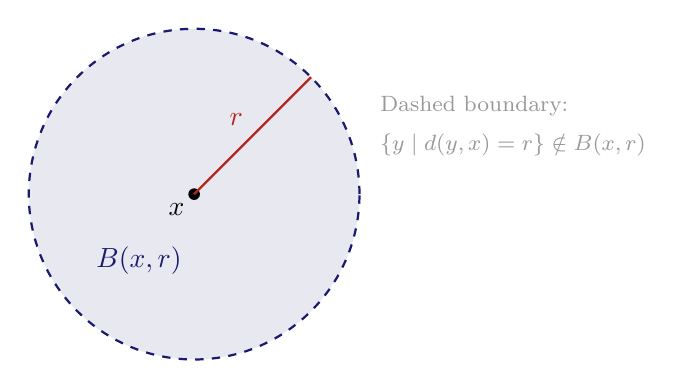
\begin{tikzpicture}[scale=1.4]
% \begin{hidden}
% - Canvas: scale 1.4, origin at (0, 0), radius r = 1.5. Footprint x in [-1.8, 2.5], y in [-1.8, 1.8].
% - Elements:
%   1. Shaded interior disk in MidnightBlue!10.
%   2. Dashed boundary circle of radius r = 1.5 in MidnightBlue.
%   3. Center point x at (0, 0).
%   4. Radial line from (0, 0) to border (45:1.5) in BrickRed.
%   5. Labels for x, r, B(x, r), and boundary note.
% - Coordinates:
%   Center: (0, 0)
%   Border endpoint: (45:1.5) = (1.06, 1.06)
%   Radial label: midway along segment at (0.53, 0.53) shifted above-left.
% - Collision check: Labels placed in distinct quadrants.
% \end{hidden}

    % Shaded interior disk
    \fill[MidnightBlue!10] (0,0) circle (1.5);

    % Dashed boundary circle indicating strict inequality
    \draw[thick, dashed, MidnightBlue] (0,0) circle (1.5);

    % Center point x
    \fill[black] (0,0) circle (1.5pt) node[below left] {$x$};

    % Radius segment
    \draw[thick, BrickRed] (0,0) -- (45:1.5);
    \node[BrickRed, above left] at (45:0.75) {$r$};

    % Label of the ball
    \node[MidnightBlue, font=\bfseries] at (-0.5, -0.6) {$B(x, r)$};

    % Annotation regarding the dashed boundary
    \node[gray!80, font=\footnotesize, anchor=west] at (1.6, 0.8) {Dashed boundary:};
    \node[gray!80, font=\footnotesize, anchor=west] at (1.6, 0.45) {$\{y \mid d(y, x) = r\} \notin B(x, r)$};
\end{tikzpicture}
\end{center}

\begin{steps}[Strict Boundary Exclusion]
The dashed circumference represents the sphere $S(x, r) := \{y \in X \mid d(y, x) = r\}$. Because the defining condition is strictly $d(y, x) < r$, points residing on this boundary circumference do not belong to the open ball $B(x, r)$.
\end{steps}
\end{content}

\subsection{Definition of Open Sets}

\begin{speech}[00:04:52 - 00:05:52]
Now, the next definition \inlinemetanote{writes \qt{defn (open \& closed sets)}} is open and closed sets. Open and closed sets.

We say that a set $U$ --- a set $U$ of my metric space $X$ --- is open \inlinemetanote{writes \qt{$\bullet$ $U \subset X$ is open}} if for every $x$ in $U$, there exists some positive radius $r$, possibly depending on $x$, such that the ball of radius $r$ centered at $x$ is contained in $U$. \inlinemetanote{writes \qt{if $\forall x \in U \ \exists r > 0 \text{ st } B(x, r) \subset U$}}
\end{speech}

\begin{content}
\begin{definition}[Open Set]\label[definition]{def:open-set}
Let $(X, d)$ be a metric space. A subset $U \subseteq X$ is called an \newterm{open set} if around every point of $U$, there exists an open ball entirely contained within $U$:
\begin{equation}\label{eq:open-set-def}
\forall x \in U \ \exists r > 0 \colon \quad B(x, r) \subseteq U.
\end{equation}
\end{definition}

\begin{steps}[Dependence of the Radius on the Point]
The radius $r$ in \eqref{eq:open-set-def} depends on the chosen point $x \in U$ (i.e., $r = r(x)$). As $x$ moves closer to the edge or boundary of $U$, the permissible radius $r$ will generally need to become strictly smaller to prevent the ball from spilling outside $U$.
\end{steps}
\end{content}

\begin{speech}[00:05:52 - 00:07:12]
In $\mathbb{R}^2$, an open set is essentially any set... This is heuristically the idea, right? Then we will see concrete open sets. But it's a set that does not include its contour --- its boundary.

Again, I didn't define the boundary yet, but now you have some common-sense knowledge of what the boundary of this set is, which is this part: the skin of the set, right? If the set is the inside without the skin, it is open.

Why? Because for any point here, you can take a ball. Depending on the distance to the boundary, right? Depending on the distance to the skin, you make the ball super, super small, and it will be contained in the set. Like I said, any point in the interior will be at a positive distance from the skin, right?
\end{speech}

\begin{content}[Geometric Intuition: The \qt{Skin} of an Open Set]
Geometrically, a subset of Euclidean space $\mathbb{R}^2$ is open if it does not contain its \qt{skin} (its boundary contour). Every point in the interior of the set sits at a strictly positive distance from the boundary, allowing a sufficiently small ball to fit entirely inside.

\begin{center}
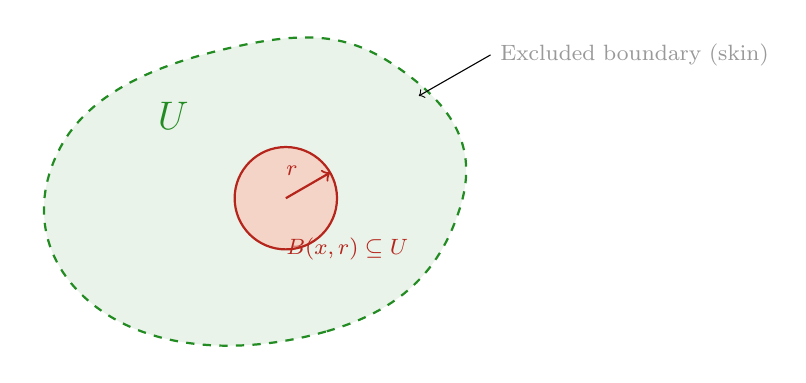
\begin{tikzpicture}[scale=1.3]
% \begin{hidden}
% - Canvas: scale 1.3, smooth closed curve representing U.
% - Elements:
%   1. Shaded interior volume of U in ForestGreen!10.
%   2. Dashed boundary representing the excluded "skin".
%   3. Point x in the interior.
%   4. Ball B(x, r) centered at x, completely inside U.
%   5. Labels and dashed distance indicator to the boundary.
% - Coordinates:
%   Control points for smooth cycle: (0, 0), (2, 0.3), (3.2, 1.2), (2.8, 2.5), (1.2, 2.8), (-0.5, 1.8).
%   Test point x: (1.5, 1.4)
%   Small radius: r = 0.45
% \end{hidden}

    % Open set boundary (dashed) and filled interior
    \fill[ForestGreen!10] plot [smooth cycle, tension=0.8] coordinates {
        (0, 0) (2.2, -0.2) (3.5, 1.0) (3.0, 2.3) (1.4, 2.6) (-0.4, 1.6)
    };
    \draw[thick, dashed, ForestGreen] plot [smooth cycle, tension=0.8] coordinates {
        (0, 0) (2.2, -0.2) (3.5, 1.0) (3.0, 2.3) (1.4, 2.6) (-0.4, 1.6)
    };

    % Set label
    \node[ForestGreen, font=\Large\bfseries] at (0.7, 1.9) {$U$};

    % Interior point x
    \coordinate (X) at (1.8, 1.1);
    \fill[black] (X) circle (1.5pt) node[below] {$x$};

    % Small open ball B(x, r) inside U
    \draw[thick, BrickRed, fill=BrickRed!15] (X) circle (0.5);
    \draw[->, thick, BrickRed] (X) -- ++(30:0.5) node[midway, above left, font=\footnotesize] {$r$};
    \node[BrickRed, font=\footnotesize] at (2.4, 0.6) {$B(x, r) \subseteq U$};

    % Annotation for the boundary
    \draw[<-] (3.1, 2.1) -- ++(0.7, 0.4) node[right, font=\footnotesize, gray!80] {Excluded boundary (\qt{skin})};
\end{tikzpicture}
\end{center}

\begin{steps}[The \qt{No Skin} Principle]
For any interior point $x \in U$, let $\delta := \inf_{y \in \partial U} d(x, y)$ denote the distance from $x$ to the boundary of $U$. Since the boundary is not part of $U$, we have $\delta > 0$. By selecting any radius $0 < r < \delta$, the entire open ball $B(x, r)$ is guaranteed to lie strictly inside $U$.
\end{steps}
\end{content}

\begin{hidden}
% timestamp: 00:06:45
% topic: Definition and geometric intuition of open sets
% board_state: def:open-ball, def:open-set
% next_goal: Demonstrate openness of the open unit square in R^2
% open_loops: none
\end{hidden}

\subsection{Example: The Open Unit Square in \texorpdfstring{$\mathbb{R}^2$}{R2}}

\begin{speech}[00:07:12 - 00:08:35]
If you want a more concrete example, take the set $(0, 1) \times (0, 1)$ \inlinemetanote{writes $(0, 1) \times (0, 1)$}, the open square, subset $\mathbb{R}^2$ \inlinemetanote{writes $\subset \mathbb{R}^2 \text{ open}$}. Prove that it is open: exercise.

You take this square \inlinemetanote{draws dashed square}, and you take a point here. A point in the square will have two coordinates. And now, what is the definition of open? If you take the point $(x_1, x_2)$ \inlinemetanote{writes $(x_1, x_2)$}, you need to construct a positive radius $r$ such that the whole ball centered at this given point belongs to the square.

In the case of the square, what is the formula for the radius? Well, you can take $r$ equal to, I don't know, something like the minimum between this distance, this distance, this distance, and this distance. So, it will be something like the minimum between $x_1$, $x_2$, $1 - x_1$, and $1 - x_2$ \inlinemetanote{writes $r = \min\{x_1, x_2, 1-x_1, 1-x_2\}$}.

You can check that this radius works --- the minimum of these four numbers, right?
\end{speech}

\begin{content}
\begin{example}[Open Unit Square in $\mathbb{R}^2$]\label[example]{ex:open-unit-square}
The Cartesian product of open intervals:
\begin{equation}\label{eq:open-square}
U := (0, 1) \times (0, 1) = \{ (x_1, x_2) \in \mathbb{R}^2 \mid 0 < x_1 < 1 \text{ and } 0 < x_2 < 1 \} \subset \mathbb{R}^2
\end{equation}
is an open subset of $(\mathbb{R}^2, d_{\text{Euc}})$.
\end{example}

\begin{proof}[Verification of Openness]
Let $x = (x_1, x_2) \in (0, 1) \times (0, 1)$. We seek a radius $r > 0$ such that $B(x, r) \subseteq (0, 1) \times (0, 1)$.
The distances from $x$ to the four boundary edges of the square are:
\begin{itemize}
    \item Distance to the left edge ($x_1 = 0$): $x_1$,
    \item Distance to the bottom edge ($x_2 = 0$): $x_2$,
    \item Distance to the right edge ($x_1 = 1$): $1 - x_1$,
    \item Distance to the top edge ($x_2 = 1$): $1 - x_2$.
\end{itemize}
Since $0 < x_1 < 1$ and $0 < x_2 < 1$, each of these four quantities is strictly positive. We define:
\begin{equation}\label{eq:min-radius-square}
r := \min \{ x_1, x_2, 1 - x_1, 1 - x_2 \} > 0.
\end{equation}
Now let $y = (y_1, y_2) \in B(x, r)$. By definition of the Euclidean metric:
\[
|y_1 - x_1| = \sqrt{(y_1 - x_1)^2} \le \sqrt{(y_1 - x_1)^2 + (y_2 - x_2)^2} = d_{\text{Euc}}(y, x) < r \le x_1,
\]
which implies $y_1 > x_1 - x_1 = 0$. Similarly:
\[
y_1 - x_1 \le |y_1 - x_1| < r \le 1 - x_1 \implies y_1 < 1.
\]
Applying the identical estimate to the second coordinate gives $0 < y_2 < 1$. Hence, $y \in (0, 1) \times (0, 1)$, confirming $B(x, r) \subseteq (0, 1) \times (0, 1)$.
\end{proof}

\begin{center}
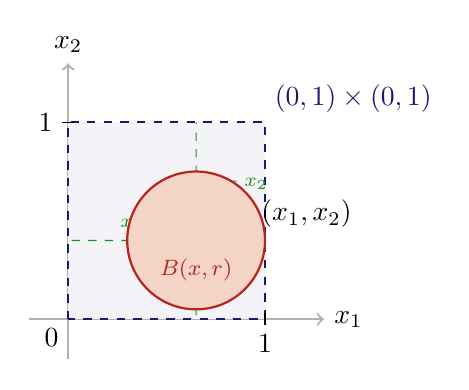
\begin{tikzpicture}[scale=2.5]
% \begin{hidden}
% - Canvas: scale 2.5, unit square [0, 1]^2.
% - Elements:
%   1. Dashed square boundary.
%   2. Interior point x = (0.65, 0.4).
%   3. Distances: x_1 = 0.65, 1 - x_1 = 0.35, x_2 = 0.40, 1 - x_2 = 0.60.
%   4. Minimum distance: r = 1 - x_1 = 0.35.
%   5. Open ball B(x, r) inscribed in the square touching the closest edge.
%   6. Four dashed projection lines showing distances to the 4 edges.
% \end{hidden}

    % Grid and axes
    \draw[->, thick, gray!60] (-0.2, 0) -- (1.3, 0) node[right, text=black] {$x_1$};
    \draw[->, thick, gray!60] (0, -0.2) -- (0, 1.3) node[above, text=black] {$x_2$};

    % Dashed open unit square
    \draw[thick, dashed, MidnightBlue, fill=MidnightBlue!5] (0, 0) rectangle (1, 1);
    \node[MidnightBlue, above right] at (1, 1) {$(0, 1) \times (0, 1)$};

    % Tick marks
    \draw (1, 0.03) -- (1, -0.03) node[below] {$1$};
    \draw (0.03, 1) -- (-0.03, 1) node[left] {$1$};
    \node[below left] at (0, 0) {$0$};

    % Interior point x
    \coordinate (X) at (0.65, 0.4);
    \fill[black] (X) circle (1.2pt) node[above right=1pt] {$x = (x_1, x_2)$};

    % Distance lines to edges
    \draw[dashed, ForestGreen] (X) -- (0, 0.4) node[midway, above, font=\scriptsize] {$x_1$};
    \draw[dashed, ForestGreen] (X) -- (0.65, 0) node[midway, right, font=\scriptsize] {$x_2$};
    \draw[dashed, ForestGreen] (X) -- (1, 0.4) node[midway, above, font=\scriptsize] {$1 - x_1$};
    \draw[dashed, ForestGreen] (X) -- (0.65, 1) node[midway, right, font=\scriptsize] {$1 - x_2$};

    % Inscribed ball with minimum radius r = min(0.65, 0.4, 0.35, 0.6) = 0.35
    \draw[thick, BrickRed, fill=BrickRed!15] (X) circle (0.35);
    \node[BrickRed, font=\footnotesize] at (0.65, 0.25) {$B(x, r)$};
\end{tikzpicture}
\end{center}
\end{content}

\section{Closed Sets and Topology}

\subsection{Closed Sets}

\begin{speech}[00:08:35 - 00:09:15]
Okay, the second point in the definition is what a closed set is.

A subset $A \subseteq X$ is called closed if the complement is open: $X \setminus A$ is open. \inlinemetanote{writes \qt{$\bullet$ $A \subset X$ is closed if $X \setminus A$ is open}}
\end{speech}

\begin{content}
\begin{definition}[Closed Set]\label[definition]{def:closed-set}
Let $(X, d)$ be a metric space. A subset $A \subseteq X$ is called a \newterm{closed set} if its complement in $X$ is open:
\begin{equation}\label{eq:closed-set-def}
A \text{ is closed} \iff X \setminus A \text{ is open}.
\end{equation}
\end{definition}

\begin{steps}[Complementary Duality]
Closedness is defined directly through openness. A set is not merely \qt{not open}; rather, a set is closed precisely when its complement contains an open ball around each of its points.
\end{steps}
\end{content}

\begin{speech}[00:09:15 - 00:10:15]
This is closed; this is open.

Now, this set is not closed, as you can show. Instead, this set, for instance, is closed: $[0, 1] \times [0, 1]$ \inlinemetanote{writes $[0, 1] \times [0, 1]$}.

Now it needs to contain the skin to be closed, because when you pass to the complement, which is by definition open, it must not contain the boundary, right?

So, the closed sets, we draw them with their skin. This is closed, $A$. \inlinemetanote{draws solid square labeled $A$}
\end{speech}

\begin{content}
\begin{example}[Closed Unit Square in $\mathbb{R}^2$]\label[example]{ex:closed-unit-square}
The closed unit square:
\[
A := [0, 1] \times [0, 1] = \{ (x_1, x_2) \in \mathbb{R}^2 \mid 0 \le x_1 \le 1 \text{ and } 0 \le x_2 \le 1 \}
\]
is a closed subset of $\mathbb{R}^2$.
\end{example}

\begin{center}
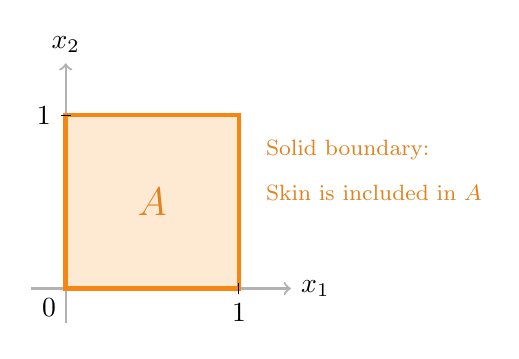
\begin{tikzpicture}[scale=2.2]
% \begin{hidden}
% - Canvas: scale 2.2, closed square [0, 1]^2 with solid boundary.
% - Elements:
%   1. Shaded square interior in BurntOrange!15.
%   2. Solid, thick yellow/BurntOrange border indicating the included "skin".
%   3. Centered label A.
%   4. Ticks and labels at 0 and 1.
% \end{hidden}
    \draw[->, thick, gray!60] (-0.2, 0) -- (1.3, 0) node[right, text=black] {$x_1$};
    \draw[->, thick, gray!60] (0, -0.2) -- (0, 1.3) node[above, text=black] {$x_2$};

    % Solid, thick boundary and filled interior
    \draw[ultra thick, BurntOrange, fill=BurntOrange!15] (0, 0) rectangle (1, 1);
    \node[BurntOrange!90!black, font=\Large\bfseries] at (0.5, 0.5) {$A$};

    % Ticks
    \draw (1, 0.03) -- (1, -0.03) node[below] {$1$};
    \draw (0.03, 1) -- (-0.03, 1) node[left] {$1$};
    \node[below left] at (0, 0) {$0$};

    % Annotation
    \node[BurntOrange!90!black, font=\footnotesize, anchor=west] at (1.1, 0.8) {Solid boundary:};
    \node[BurntOrange!90!black, font=\footnotesize, anchor=west] at (1.1, 0.55) {Skin is included in $A$};
\end{tikzpicture}
\end{center}

\begin{steps}[Why the Closed Square Has an Open Complement]
The complement $\mathbb{R}^2 \setminus ([0, 1] \times [0, 1])$ is the union of four unbounded open half-planes:
\[
\{x_1 < 0\} \cup \{x_1 > 1\} \cup \{x_2 < 0\} \cup \{x_2 > 1\}.
\]
Since each of these half-planes is open, their union is open, proving that the square $[0, 1] \times [0, 1]$ is closed.
\end{steps}
\end{content}

\subsection{The Topology Associated to a Metric}

\begin{speech}[00:10:15 - 00:11:35]
And maybe the last part of this definition, which we will not actually use, but it is a common term that you will find in books and it's good that you know, is what a topology is. \inlinemetanote{writes \qt{Topology associated to $d$}}

You will see in the notes the word \qt{topology} many times. You are not yet studying topology, but just for your information, the topology associated to the distance $d$ is --- we can put a $\mathcal{T}$ like this, a sort of calligraphic $\mathcal{T}$ --- the collection of all open sets: \inlinemetanote{writes $\mathcal{T} = \{ U \subset X \mid U \text{ open} \}$}

This is the topology. So, when we say that something is a topological notion, it has to do with this collection of open sets.
\end{speech}

\begin{content}
\begin{definition}[Metric Topology]\label[definition]{def:metric-topology}
Let $(X, d)$ be a metric space. The \newterm{topology associated to $d$} (or metric topology) is the collection $\mathcal{T}$ of all open subsets of $X$:
\begin{equation}\label{eq:metric-topology-def}
\mathcal{T} := \{ U \subseteq X \mid U \text{ is open in } (X, d) \}.
\end{equation}
\end{definition}

\begin{steps}[Topological Properties]
Any mathematical property that can be defined purely in terms of the collection $\mathcal{T}$ (without directly referring to the numerical distances $d(x, y)$) is called a \newterm{topological property}. These include openness, closedness, continuity, compactness, and connectedness.
\end{steps}
\end{content}

\begin{hidden}
% timestamp: 00:12:15
% topic: Properties of open sets: arbitrary unions and finite intersections
% board_state: def:open-set, def:closed-set, def:metric-topology, lem:unions-intersections-open
% next_goal: Prove that arbitrary unions of open sets are open
% open_loops: student distraction regarding exam results
\end{hidden}

\section{Properties of Open and Closed Sets}

\subsection{Unions and Intersections of Open Sets}

\begin{speech}[00:11:35 - 00:12:55]
Now, because this is still a bit abstract, to see a bit more practically how we identify open and closed sets, we are going to do it through sequences, okay?

Well, let me first do a lemma that we will use many times. Lemma: unions and intersections of open sets. \inlinemetanote{writes \qt{Lemma ($\cup, \cap$ of open sets)}}

This is one of the basic properties. It's very simple, but since we will use it many, many times, I will prove it now. It says that --- I will put it in words first, and then we will prove it with symbols --- arbitrary unions of open sets are open. \inlinemetanote{writes \qt{$\bullet$ Arbitrary unions of open sets are open}}
\end{speech}

\begin{speech}[00:12:55 - 00:13:17]
I'm sorry, there is a bit of discussion. Would someone tell me what is going on? Who? Who's brave enough? Ah, good.
\end{speech}

\begin{student}[Student Remark: Exam Results]
I think we're waiting for the results. \inlinemetanote{laughter}
\end{student}

\begin{speech}[00:13:21 - 00:13:24]
For results of what?
\end{speech}

\begin{student}[Student Remark, continued]
From exams... exams...
\end{student}

\begin{speech}[00:13:26 - 00:13:27]
Ah, of some exam?
\end{speech}

\begin{student}[Student Remark, continued]
Yeah.
\end{student}

\begin{speech}[00:13:28 - 00:14:09]
Ah, okay! So, it's not that you are not following... \inlinemetanote{laughter from the classroom} Okay, good.

So, this means that... So, today is the result of the first exams of the first semester? Okay, I can see that you are stressed, then. \inlinemetanote{laughter}

Could we try to be stressed in a lower voice? \inlinemetanote{laughter} Because otherwise, it will be a bit difficult.
\end{speech}

\begin{speech}[00:14:09 - 00:15:45]
So, arbitrary unions of open sets are open. This means that if you have some collection $\{U_i\}_{i \in I}$ \inlinemetanote{writes $\{U_i\}_{i \in I}$} of open subsets $U_i \subset X$ \inlinemetanote{writes $U_i \subset X \text{ open}$}, then the union of this collection is also open, right? \inlinemetanote{writes $\bigcup_{i \in I} U_i \text{ is open}$}

And also, finite intersections of open sets are open, right? \inlinemetanote{writes \qt{$\bullet$ Finite intersections of open sets are open}} This means that if $I$ is a finite set --- let's put it like this: the intersection of $U_i$ for $i$ from $1$ to capital $N$, a bounded number --- this is an open set. \inlinemetanote{writes $\bigcap_{i=1}^N U_i \text{ open}$ }
\end{speech}

\begin{content}
\begin{lemma}[Unions and Intersections of Open Sets]\label[lemma]{lem:unions-intersections-open}
Let $(X, d)$ be a metric space.
\begin{enumerate}[label=\textbf{(\roman*)}]
    \item \textbf{Arbitrary Unions:} If $\{U_i\}_{i \in I}$ is any arbitrary (finite or infinite) collection of open sets in $X$, then their union is open:
    \begin{equation}\label{eq:arbitrary-unions-open}
    \bigcup_{i \in I} U_i \text{ is open}.
    \end{equation}
    \item \textbf{Finite Intersections:} If $U_1, \dots, U_N$ is a finite collection of open sets in $X$, then their intersection is open:
    \begin{equation}\label{eq:finite-intersections-open}
    \bigcap_{i=1}^N U_i \text{ is open}.
    \end{equation}
\end{enumerate}
\end{lemma}
\end{content}

\begin{proofWrapper}[Proof of Lemma \ref{lem:unions-intersections-open}]

\begin{speech}[00:15:45 - 00:17:40]
The proof of this is just using the definition. \inlinemetanote{writes \qt{proof}}

If I want to check that a union is open, I take a point $x$ in this set that is the union: \inlinemetanote{writes \qt{take $x \in \bigcup_{i \in I} U_i$}} Then, in particular, $x$ belongs to one of them, because it's a union. I call it $i_0$ --- it's one of the indices $i$, any of them. \inlinemetanote{writes $\implies x \in U_{i_0}$} And then, since this set is open by the statement, there exists some radius $r > 0$ \inlinemetanote{writes $\implies \exists r > 0$} such that the ball of radius $r$ centered at $x$ is contained in $U_{i_0}$. But this is contained in the union of the $U_i$'s: \inlinemetanote{writes $\text{st } B(x, r) \subset U_{i_0} \subset \bigcup_{i \in I} U_i$} which proves that this union is open, right?
\end{speech}

\begin{content}[Proof of Part (i): Arbitrary Unions]
Let $x \in \bigcup_{i \in I} U_i$.
By definition of the union, there exists an index $i_0 \in I$ such that:
\[
x \in U_{i_0}.
\]
Since $U_{i_0}$ is open, there exists a radius $r > 0$ such that:
\[
B(x, r) \subseteq U_{i_0}.
\]
Since $U_{i_0} \subseteq \bigcup_{i \in I} U_i$, it follows immediately that:
\[
B(x, r) \subseteq U_{i_0} \subseteq \bigcup_{i \in I} U_i.
\]
Since $x$ was arbitrary, this proves that $\bigcup_{i \in I} U_i$ is open.
\end{content}

\begin{speech}[00:17:40 - 00:18:04]
With the finite intersection, you can do it as an exercise. But I will tell you how to do it, okay? Now I will explain the proof with... Yeah? \inlinemetanote{throws catch-box microphone to a student}
\end{speech}

\begin{student}[Student Question: Clopen Sets]
Hello? Yeah. My question was: except for the empty set and the set $X$ itself, can you give us some examples of both closed and open sets?
\end{student}

\begin{speech}[00:18:16 - 00:19:06]
We will discuss this when we discuss connected spaces, okay? This is a good question.

The whole space and the empty set are always open and closed, and I will emphasize this when we see connected spaces. So, you need to wait a bit more. I could give an example, but it's not very interesting --- it's just a disconnected space, like the disjoint union of two intervals or something like this, where each interval is open and closed.

But this would not be very interesting. You will see the interest of this question when we see connected spaces, okay? But it's a fair question.
\end{speech}

\begin{speech}[00:19:06 - 00:20:34]
So, I am saying that when you take open sets... \inlinemetanote{catches microphone back} When you take finitely many intersections of open sets, you get something open. Why? I will say it in words, and then you try to write it down, okay?

You have finitely many open sets. And now you take a point that is in the intersection of these finitely many, right? This means that the point is in all of them, right? And now, for each of the sets, you pick a radius --- which is different every time --- but there are finitely many radii such that you can put your ball inside the open set. If you take the minimum of all these radii, it will be good: with the minimum of the finitely many radii, you will fall inside the intersection.

Okay? You don't need to understand what I just said right away; please try to do the exercise. If there are problems doing this, you have it in the notes. But I think it is very good to try these first proofs of the theory, which are very short, one-line proofs. It's a very good opportunity to do it as an exercise to see if we understood the definitions, because it's one line, so you don't need to think too much. Okay.
\end{speech}

\begin{content}[Proof of Part (ii): Finite Intersections]
Let $U_1, \dots, U_N$ be open sets in $X$, and let $x \in \bigcap_{i=1}^N U_i$.
By definition of the intersection:
\[
x \in U_i \quad \text{for every } i \in \{1, \dots, N\}.
\]
Since each $U_i$ is open, there exist radii $r_1, \dots, r_N > 0$ such that:
\[
B(x, r_i) \subseteq U_i \quad \text{for each } i \in \{1, \dots, N\}.
\]
We define the radius:
\begin{equation}\label{eq:min-radius-intersection}
r := \min \{ r_1, r_2, \dots, r_N \}.
\end{equation}
Since the set $\{r_1, \dots, r_N\}$ is finite and each $r_i > 0$, its minimum is strictly positive: $r > 0$.
Now, since $r \le r_i$ for all $i \in \{1, \dots, N\}$, we have:
\[
B(x, r) \subseteq B(x, r_i) \subseteq U_i \quad \text{for every } i \in \{1, \dots, N\}.
\]
Consequently, the ball is contained in all $U_i$ simultaneously:
\[
B(x, r) \subseteq \bigcap_{i=1}^N U_i.
\]
This proves that $\bigcap_{i=1}^N U_i$ is open.

\begin{steps}[Why Finiteness is Essential for Intersections]
The positivity of $r = \min\{r_1, \dots, r_N\}$ relies fundamentally on taking the minimum over a \emph{finite} number of strictly positive elements. For an infinite collection of open sets, the infimum of positive radii can equal zero:
\[
\inf_{n \in \mathbb{N}} \left\{ \frac{1}{n} \right\} = 0.
\]
For example, in $\mathbb{R}$ with open intervals $U_n = \left(-\frac{1}{n}, \frac{1}{n}\right)$, their infinite intersection is a single point:
\[
\bigcap_{n=1}^\infty \left(-\frac{1}{n}, \frac{1}{n}\right) = \{0\},
\]
which is not open.
\end{steps}
\end{content}

\end{proofWrapper}

\subsection{Unions and Intersections of Closed Sets}

\begin{speech}[00:20:34 - 00:22:04]
Now, an analogous lemma, but for closed sets: Lemma: unions and intersections of closed sets. \inlinemetanote{writes \qt{Lemma ($\cup, \cap$ of closed sets)}}

And it's the same, but the opposite. It says that finite unions of closed sets are closed \inlinemetanote{writes \qt{$\bullet$ Finite unions of closed sets are closed}}, and arbitrary intersections --- it could be finite or infinite --- of closed sets are closed, okay? \inlinemetanote{writes \qt{$\bullet$ Arbitrary intersections of closed sets are closed}}

You can repeat the same proof, or a variant of the same proof, or you can reason by passing to the complement. Remember that being closed is defined as the complement being open. If you pass to the complement, complementation converts closed sets into open sets, and open sets into closed sets, right?

So, you can always pass statements about open sets to the complement, and you get a statement about closed sets. If you have some property of open sets and you pass the whole statement to the complements, you get a property of closed sets.
\end{speech}

\begin{content}
\begin{lemma}[Unions and Intersections of Closed Sets]\label[lemma]{lem:unions-intersections-closed}
Let $(X, d)$ be a metric space.
\begin{enumerate}[label=\textbf{(\roman*)}]
    \item \textbf{Finite Unions:} If $A_1, \dots, A_N$ is a finite collection of closed sets in $X$, then their union is closed:
    \begin{equation}\label{eq:finite-unions-closed}
    \bigcup_{i=1}^N A_i \text{ is closed}.
    \end{equation}
    \item \textbf{Arbitrary Intersections:} If $\{A_i\}_{i \in I}$ is any arbitrary (finite or infinite) collection of closed sets in $X$, then their intersection is closed:
    \begin{equation}\label{eq:arbitrary-intersections-closed}
    \bigcap_{i \in I} A_i \text{ is closed}.
    \end{equation}
\end{enumerate}
\end{lemma}
\end{content}

\begin{speech}[00:22:04 - 00:23:55]
And this is what we have here. Why? Because $X$ minus a union of sets \inlinemetanote{writes $X \setminus \bigcup_{i \in I} A_i$} is the same as the intersection of the complements, right? \inlinemetanote{writes $= \bigcap_{i \in I} (X \setminus A_i)$} When you take the complement of a union, you get the intersection of the complements.

And the same: the complement of an intersection \inlinemetanote{writes $X \setminus \bigcap_{i \in I} A_i$} is equal to the union of the complements. \inlinemetanote{writes $= \bigcup_{i \in I} (X \setminus A_i)$}

Then you apply the previous result. You apply this property of how intersections pass to unions when you complement, and vice versa, and then you apply the previous result. Because if these sets are closed, these sets will be open, and the finite intersection of open sets is open, okay?
\end{speech}

\begin{content}[Proof via De Morgan's Laws]
\begin{proof}[Proof of \cref{lem:unions-intersections-closed}]
We use De Morgan's laws to translate the properties of open sets directly to closed sets:

\textbf{Proof of Part (i) (Finite Unions):}
Let $A_1, \dots, A_N$ be closed sets. By definition, each complement $X \setminus A_i$ is open.
By De Morgan's law:
\begin{equation}\label{eq:demorgan-union}
X \setminus \left( \bigcup_{i=1}^N A_i \right) = \bigcap_{i=1}^N (X \setminus A_i).
\end{equation}
By \cref{lem:unions-intersections-open} part \textbf{(ii)}, the finite intersection of open sets $\bigcap_{i=1}^N (X \setminus A_i)$ is open.
Therefore, the complement $X \setminus \left( \bigcup_{i=1}^N A_i \right)$ is open, which proves that $\bigcup_{i=1}^N A_i$ is closed.

\textbf{Proof of Part (ii) (Arbitrary Intersections):}
Let $\{A_i\}_{i \in I}$ be an arbitrary collection of closed sets. Then each $X \setminus A_i$ is open.
By De Morgan's law:
\begin{equation}\label{eq:demorgan-intersection}
X \setminus \left( \bigcap_{i \in I} A_i \right) = \bigcup_{i \in I} (X \setminus A_i).
\end{equation}
By \cref{lem:unions-intersections-open} part \textbf{(i)}, the arbitrary union of open sets $\bigcup_{i \in I} (X \setminus A_i)$ is open.
Therefore, the complement $X \setminus \left( \bigcap_{i \in I} A_i \right)$ is open, which proves that $\bigcap_{i \in I} A_i$ is closed.
\end{proof}

\begin{steps}[Duality Summary: Open vs. Closed Sets]
\begin{center}
\begin{tabular}{l l}
    \textbf{Open Sets $\mathcal{T}$} & \textbf{Closed Sets} \\
    \hline
    Arbitrary unions are open & Finite unions are closed \\
    Finite intersections are open & Arbitrary intersections are closed \\
\end{tabular}
\end{center}
De Morgan's laws swap unions and intersections upon complementation, directly exchanging the roles of arbitrary and finite operations.
\end{steps}
\end{content}

\begin{hidden}
% timestamp: 00:23:50
% topic: Lemma on closed set unions and intersections via De Morgan's laws
% board_state: lem:unions-intersections-closed, eq:demorgan-union, eq:demorgan-intersection
% next_goal: Sequences and characterization of closed sets via limits
% open_loops: none
\end{hidden}

\subsection{Importance of Finiteness: Infinite Intersections and Unions}

\begin{speech}[00:23:54 - 00:25:17]
Okay. What else...

Let me give an example, very, very easy, showing that this property --- where we said finite intersections or finite unions --- is important that it is finite. When you take infinite intersections of open sets, you can get a closed set that is not open.

Example: finite is important. \inlinemetanote{writes \qt{Example (finite is important)}}

If you take one of the spaces that you are most familiar with, namely $\mathbb{R}$ with the distance given by the absolute value \inlinemetanote{writes $(\mathbb{R}, d_{|\cdot|})$} --- with the Euclidean distance --- and you take the sets $U_k = (-1/k, 1/k)$ \inlinemetanote{writes $U_k = (-1/k, 1/k)$}, and you take their intersection: then the intersection for $k$ from $1$ to infinity of $U_k$ \inlinemetanote{writes $\bigcap_{k=1}^\infty U_k$} gives you the point zero: \inlinemetanote{writes $= \{0\}$}
\end{speech}

\begin{speech}[00:25:17 - 00:26:14]
These are open intervals, and since the intervals do not contain their endpoints, each of them is open. But when you take their intersection, you get just the point zero, and the point zero is not open, because you cannot put any ball in it, right? The point zero is closed, but it is not open.

So, these are open, and this is not open. \inlinemetanote{writes \qt{open} next to $U_k$ and \qt{not open!} next to $\{0\}$}

That's why it is important that the intersection is of finitely many sets. And passing to the complement, you get a counterexample for infinite unions of closed sets.

Any questions about this?
\end{speech}

\begin{content}
\begin{example}[Infinite Intersection of Open Sets Need Not Be Open]\label[example]{ex:infinite-intersection-not-open}
In $(\mathbb{R}, d_{\text{Euc}})$, consider the family of open intervals indexed by $k \in \mathbb{N}_{\ge 1}$:
\begin{equation}\label{eq:nested-open-intervals}
U_k := \left( -\frac{1}{k}, \frac{1}{k} \right) \quad (\text{open}).
\end{equation}
Taking the infinite intersection over all $k \ge 1$ yields:
\begin{equation}\label{eq:infinite-intersection-zero}
\bigcap_{k=1}^\infty U_k = \{ 0 \} \quad (\text{not open!}).
\end{equation}
\end{example}

\begin{steps}[Why the Singleton $\{0\}$ is Closed but Not Open]
\begin{itemize}
    \item \textbf{$\{0\}$ is not open:} For any radius $r > 0$, the open ball centered at $0$ is the interval $B(0, r) = (-r, r)$. For any $r > 0$, $(-r, r) \not\subseteq \{0\}$ because it contains non-zero points (e.g., $r/2$). Thus, no open ball around $0$ is contained in $\{0\}$.
    \item \textbf{$\{0\}$ is closed:} Its complement $\mathbb{R} \setminus \{0\} = (-\infty, 0) \cup (0, \infty)$ is an arbitrary union of two open intervals, hence open in $\mathbb{R}$.
    \item \textbf{Dual Counterexample via Complements:} Taking the complements $A_k := \mathbb{R} \setminus U_k = (-\infty, -1/k] \cup [1/k, \infty)$ yields an infinite family of closed sets whose union:
    \[
    \bigcup_{k=1}^\infty A_k = \mathbb{R} \setminus \bigcap_{k=1}^\infty U_k = \mathbb{R} \setminus \{0\}
    \]
    is open, and hence not closed. This demonstrates that arbitrary unions of closed sets need not be closed.
\end{itemize}
\end{steps}
\end{content}

\begin{hidden}
% timestamp: 00:06:15
% topic: De Morgan duality and counterexample to infinite intersection of open sets
% board_state: lem:unions-intersections-closed, ex:infinite-intersection-not-open
% next_goal: Define interior, closure, and boundary in an arbitrary metric space
% open_loops: none
\end{hidden}

\section{Interior, Closure, and Boundary in Metric Spaces}

\subsection{Definitions of Interior, Closure, and Boundary}

\begin{speech}[00:26:14 - 00:27:44]
Now we will define something interesting, which is what we were saying earlier heuristically: what the interior and the boundary of a set in a topological space are.

In a metric space: \inlinemetanote{writes \qt{Defn (Interior, bdry, in metric space)} on the middle board} Given a set... Let me call the set $Y \subset X$ \inlinemetanote{writes \qt{Given $Y \subset X$}}, $(X, d)$ a metric space \inlinemetanote{writes $(X, d) \text{ metric space}$}. Should I call it $Y$, or let me call it... I don't know, later $Y$ will be something else. $\Omega$, whatever. \inlinemetanote{erases $Y$ and writes $\Omega \subset X$}

Given a set in my metric space,
\end{speech}

\begin{speech}[00:27:44 - 00:29:19]
I define the interior of $\Omega$: \inlinemetanote{writes \qt{$\bullet$ $\operatorname{int}(\Omega) =$}} Maybe I will not put parentheses; I will say $\operatorname{int} \Omega$, or sometimes you put $\Omega$ with a circle like this \inlinemetanote{writes $\Omega^\circ$}, depending on the source. This is what is called the interior of $\Omega$. \inlinemetanote{underlines and writes \qt{interior of $\Omega$}}

This is, by definition, the largest open set contained in $\Omega$. You have your set $\Omega$, you look at all the open sets that are contained in it, and the largest one is the union of all open sets contained in $\Omega$. That is, the union of $U \subset \Omega$ such that $U$ is open: \inlinemetanote{writes $= \bigcup \{ U \subset \Omega \mid U \text{ is open} \}$}

Right? This is the interior.
\end{speech}

\begin{content}
\begin{definition}[Interior of a Set]\label[definition]{def:interior-set}
Let $(X, d)$ be a metric space and $\Omega \subseteq X$ an arbitrary subset. The \newterm{interior} of $\Omega$, denoted by $\operatorname{int}(\Omega)$ or $\Omega^\circ$, is defined as the union of all open subsets of $X$ contained in $\Omega$:
\begin{equation}\label{eq:interior-def}
\operatorname{int}(\Omega) = \Omega^\circ := \bigcup \{ U \subseteq \Omega \mid U \text{ is open in } (X, d) \}.
\end{equation}
\end{definition}

\begin{steps}[Characterization of the Interior]
\begin{itemize}
    \item \textbf{Openness:} Since $\Omega^\circ$ is an arbitrary union of open sets, it is itself open by \cref{lem:unions-intersections-open}.
    \item \textbf{Largest Open Subset:} If $V \subseteq \Omega$ is any open set, then $V$ is one of the sets in the union \eqref{eq:interior-def}, so $V \subseteq \Omega^\circ$. Thus, $\Omega^\circ$ is the unique maximal open subset of $\Omega$.
    \item \textbf{Openness Criterion:} A set $\Omega$ is open if and only if $\Omega = \Omega^\circ$.
\end{itemize}
\end{steps}
\end{content}

\begin{speech}[00:29:19 - 00:30:44]
Now, I also define the closure, which you know from $\mathbb{R}$, right? The closure of some set is the set of points $x \in X$ such that there exists some sequence $(x_n)$ contained inside the set $\Omega$, and the sequence converges to $x$: \inlinemetanote{writes $\bullet \ \overline{\Omega} = \{ x \in X \mid \exists (x_n)_{n \ge 0} \subset \Omega, \ x_n \to x \}$}
\end{speech}

\begin{content}
\begin{definition}[Closure of a Set via Sequences]\label[definition]{def:closure-set-sequences}
Let $(X, d)$ be a metric space and $\Omega \subseteq X$. The \newterm{closure} of $\Omega$, denoted by $\overline{\Omega}$, is defined as the set of all limit points of sequences in $\Omega$:
\begin{equation}\label{eq:closure-sequential-def}
\overline{\Omega} := \{ x \in X \mid \exists (x_n)_{n \ge 0} \subseteq \Omega \text{ such that } x_n \to x \}.
\end{equation}
\end{definition}
\end{content}

\begin{speech}[00:30:44 - 00:32:34]
Here I can do a drawing, right? Let's look at an example. \inlinemetanote{moves to the right chalkboard and writes \qt{Example $[0, 1) \times [0, 1) = \Omega$}} Let's take this example: say, $[0, 1) \times [0, 1)$ --- closed-open, closed-open.

How do you draw this example? It would be something like this, right? \inlinemetanote{draws a square with solid bottom and left edges, dashed top and right edges, and hatched interior} It is the inside of this square, but you are missing this part of the boundary and this part of the boundary.

Now, can you see that these points satisfy this definition here? If I take a point $x$ here on the boundary --- sorry, on the closure --- because I can take a sequence of points from the inside, from the red part (i.e., the hatched interior), that approaches $x$, right? But these points that are not in my set, because I am excluding them, are also in the closure. This point $x$ over here is also in the closure. \inlinemetanote{draws point $x$ on the dashed top edge with sequence dots approaching it, labeled $\cdot \to x \in \overline{\Omega}$} This belongs to the closure because I can take a sequence from here that approaches my point, right?

You can also define this --- and actually we will prove this --- as the intersection of all closed sets that are bigger than $\Omega$: \inlinemetanote{writes $= \bigcap \{ A \supset \Omega \mid A \text{ closed}\}$ on the left board} So, the closure is the smallest closed set that contains $\Omega$.
\end{speech}

\begin{content}
\begin{definition}[Closure as Smallest Closed Superset]\label[definition]{def:closure-set-intersection}
Equivalently, the closure $\overline{\Omega}$ of $\Omega \subseteq X$ is defined as the intersection of all closed subsets of $X$ containing $\Omega$:
\begin{equation}\label{eq:closure-intersection-def}
\overline{\Omega} = \bigcap \{ A \subseteq X \mid \Omega \subseteq A \text{ and } A \text{ is closed in } (X, d) \}.
\end{equation}
\end{definition}

\begin{steps}[Equivalence of the Two Definitions of Closure]
\begin{itemize}
    \item \textbf{Smallest Closed Set:} By \cref{lem:unions-intersections-closed}, an arbitrary intersection of closed sets is closed. Hence, $\overline{\Omega}$ defined via \eqref{eq:closure-intersection-def} is closed and is the unique minimal closed set containing $\Omega$.
    \item \textbf{Closedness Criterion:} A set $\Omega$ is closed if and only if $\Omega = \overline{\Omega}$.
    \item \textbf{Equivalence with Sequences:} We will formally prove in \cref{lem:open-closed-sequences} that the sequential definition \eqref{eq:closure-sequential-def} and the topological definition \eqref{eq:closure-intersection-def} coincide in any metric space.
\end{itemize}
\end{steps}
\end{content}

\begin{speech}[00:32:34 - 00:33:29]
And their difference --- this minus that --- is called the boundary, and is denoted with this symbol, the del symbol: \inlinemetanote{writes $\bullet \ \overline{\Omega} \setminus \Omega^\circ =: \partial\Omega \longleftarrow \text{boundary of } \Omega$} This is called the boundary of $\Omega$.

And this boundary of $\Omega$ is the skin. \inlinemetanote{writes \qt{\qt{skin}}} Right? If you do any example in the plane, you will see what this is doing: the closure is taking the set with the skin, including the inside, and then for the boundary you are removing the inside.
\end{speech}

\begin{content}
\begin{definition}[Boundary of a Set]\label[definition]{def:boundary-set}
Let $(X, d)$ be a metric space and $\Omega \subseteq X$. The \newterm{boundary} of $\Omega$, denoted by $\partial\Omega$, is defined as the set difference between the closure and the interior:
\begin{equation}\label{eq:boundary-def}
\partial\Omega := \overline{\Omega} \setminus \Omega^\circ.
\end{equation}
\end{definition}

\begin{steps}[Heuristic and Topological Role of the Boundary]
Heuristically, the boundary $\partial\Omega$ is the \qt{skin} of the set. Points in $\partial\Omega$ have the property that every open neighborhood intersects both $\Omega$ and its complement $X \setminus \Omega$.
\end{steps}
\end{content}

\begin{speech}[00:33:29 - 00:35:04]
For this set over here, the interior would be this: \inlinemetanote{draws a square with all 4 dashed edges and hatched interior} This would be $\Omega^\circ$, the interior $(0, 1)^2$. \inlinemetanote{labels $\Omega^\circ$ and writes $(0, 1)^2$}

Then, when you take the closure, you also get the points that can be approximated by a sequence --- or if you take the intersection of closed sets, you get the closed square $[0, 1]^2$: \inlinemetanote{draws a square with all 4 solid edges and hatched interior, labels $[0, 1]^2$}

And if you want the boundary, it's the difference between the two, which is just this part, without the inside: \inlinemetanote{draws a hollow square with 4 solid edges and empty interior, labels $\partial\Omega$} Right?

Again, all of these are perfectly common-sense notions, but we can formalize them and make them perfectly rigorous just using these few axioms. And then... \inlinemetanote{pauses and pushes the chalkboards upward}
\end{speech}

\begin{content}
\begin{example}[Decomposition of the Half-Open Unit Square in $\mathbb{R}^2$]\label[example]{ex:square-decomposition}
Let $\Omega = [0, 1) \times [0, 1) \subset \mathbb{R}^2$. Then:
\begin{itemize}
    \item \textbf{Interior:} $\Omega^\circ = (0, 1) \times (0, 1) = (0, 1)^2$,
    \item \textbf{Closure:} $\overline{\Omega} = [0, 1] \times [0, 1] = [0, 1]^2$,
    \item \textbf{Boundary:} $\partial\Omega = \overline{\Omega} \setminus \Omega^\circ = ([0, 1] \times [0, 1]) \setminus ((0, 1) \times (0, 1))$.
\end{itemize}
\end{example}

\begin{center}
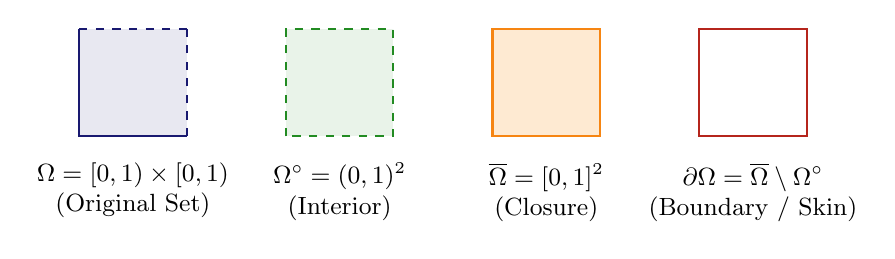
\begin{tikzpicture}[scale=1.05]
% \begin{hidden}
% - Canvas: scale=1.05, 4 square diagrams placed along x-axis with centers at x = 0, 2.5, 5.0, 7.5.
% - Elements:
%   (1) \Omega = [0, 1) x [0, 1): solid bottom/left edges, dashed top/right edges, hatched fill.
%   (2) \Omega^\circ = (0, 1)^2: all 4 edges dashed, hatched fill.
%   (3) \overline{\Omega} = [0, 1]^2: all 4 edges solid, hatched fill.
%   (4) \partial\Omega: all 4 edges solid, completely empty interior.
% - Coordinates: square size 1.3 x 1.3 centered at y = 0.
%   Square 1: x in [-0.65, 0.65], y in [-0.65, 0.65].
%   Square 2: x in [1.85, 3.15], y in [-0.65, 0.65].
%   Square 3: x in [4.35, 5.65], y in [-0.65, 0.65].
%   Square 4: x in [6.85, 8.15], y in [-0.65, 0.65].
% - Labels: positioned below each square at y = -1.05.
% - Collisions: horizontal separation of 1.2 cm between squares ensures zero collision.
% \end{hidden}

    % 1. The Set \Omega
    \fill[MidnightBlue!10] (-0.65, -0.65) rectangle (0.65, 0.65);
    \draw[thick, dashed, MidnightBlue] (-0.65, 0.65) -- (0.65, 0.65);
    \draw[thick, dashed, MidnightBlue] (0.65, -0.65) -- (0.65, 0.65);
    \draw[thick, MidnightBlue] (-0.65, 0.65) -- (-0.65, -0.65) -- (0.65, -0.65);
    \node[below, font=\small, align=center] at (0, -0.85) {$\Omega = [0, 1) \times [0, 1)$\\(Original Set)};

    % 2. Interior \Omega^\circ
    \begin{scope}[shift={(2.5, 0)}]
        \fill[ForestGreen!10] (-0.65, -0.65) rectangle (0.65, 0.65);
        \draw[thick, dashed, ForestGreen] (-0.65, -0.65) rectangle (0.65, 0.65);
        \node[below, font=\small, align=center] at (0, -0.85) {$\Omega^\circ = (0, 1)^2$\\(Interior)};
    \end{scope}

    % 3. Closure \overline{\Omega}
    \begin{scope}[shift={(5.0, 0)}]
        \fill[BurntOrange!15] (-0.65, -0.65) rectangle (0.65, 0.65);
        \draw[thick, BurntOrange] (-0.65, -0.65) rectangle (0.65, 0.65);
        \node[below, font=\small, align=center] at (0, -0.85) {$\overline{\Omega} = [0, 1]^2$\\(Closure)};
    \end{scope}

    % 4. Boundary \partial\Omega
    \begin{scope}[shift={(7.5, 0)}]
        \draw[thick, BrickRed] (-0.65, -0.65) rectangle (0.65, 0.65);
        \node[below, font=\small, align=center] at (0, -0.85) {$\partial\Omega = \overline{\Omega} \setminus \Omega^\circ$\\(Boundary / \qt{Skin})};
    \end{scope}
\end{tikzpicture}
\end{center}
\end{content}

\begin{hidden}
% timestamp: 00:15:05
% topic: Definition of interior, closure, boundary and the unit square example
% board_state: def:interior-set, def:closure-set-sequences, def:closure-set-intersection, def:boundary-set, ex:square-decomposition
% next_goal: State and prove the lemma characterizing open and closed sets through convergent sequences
% open_loops: none
\end{hidden}

\section{Sequential Characterization of Open and Closed Sets}

\subsection{Statement of the Lemma}

\begin{speech}[00:35:04 - 00:36:04]
Now, I gave two different definitions of the closure: one through sequences --- points that can be approximated by a sequence from the set --- and one that is the intersection of all closed sets that contain my set, right? And I said these are the same.

I'm going to give a lemma that actually shows that these are the same. After this lemma, you can take whichever of the two definitions is more convenient each time.

This lemma is called \qt{open and closed sets through sequences}: how we determine if a set is open or closed using convergent sequences. \inlinemetanote{writes \qt{Lemma (open \& closed through sequences)} on the lower left chalkboard}
\end{speech}

\begin{speech}[00:36:04 - 00:37:39]
It says that $U$ --- I don't write it every time, but throughout all this chapter, every time it should say $(X, d)$ is a metric space, right? \inlinemetanote{writes $(X, d) \text{ ms}$}

A subset $U \subseteq X$ is open if and only if, whenever I have a sequence $x_n$ in my space and $x_n$ converges to a point $x \in U$, then $x_n$ belongs to $U$ for all $n$ up to finitely many exceptions: \inlinemetanote{writes \qt{(1) $U \subset X$ open $\iff$ [ whenever $(x_n)_{n \ge 0} \subset X$, $x_n \to x \in U \implies x_n \in U$ for all $n$ up to finitely many exceptions ]}}
\end{speech}

\begin{content}
\begin{lemma}[Sequential Characterization of Open and Closed Sets]\label[lemma]{lem:open-closed-sequences}
Let $(X, d)$ be a metric space.
\begin{enumerate}[label=\textbf{(\arabic*)}]
    \item \textbf{Open Sets:} A subset $U \subseteq X$ is open if and only if for every sequence $(x_n)_{n \ge 0} \subseteq X$ converging to a point $x \in U$, the sequence belongs to $U$ for all $n$ up to finitely many exceptions:
    \begin{equation}\label{eq:seq-open-def}
    U \subseteq X \text{ is open} \iff \left[ \begin{aligned} &\text{whenever } (x_n)_{n \ge 0} \subseteq X \text{ with } x_n \to x \in U, \\ &\implies x_n \in U \text{ for all } n \text{ up to finitely many exceptions} \end{aligned} \right].
    \end{equation}
\end{enumerate}
\end{lemma}
\end{content}

\begin{speech}[00:37:39 - 00:38:59]
You see, I'm going to do the drawing. \inlinemetanote{draws a sketch of an open set $U$ with dashed boundary and an incoming sequence $x_n$ converging to $x \in U$} This is my drawing of an open set $U$. I have some sequence in the space that is going to converge to this point. It could start anywhere, but it is going to converge to this point. So, after finitely many exceptions, you will be inside the open set.

Why? Because the open set always contains a ball, and the definition of convergence means that at some point you will be inside this ball, whatever the radius of the ball is. This is exactly the definition of convergence.

And this will be the proof, which I will write down, right? This is almost a proof with a picture. You need to translate this picture into symbols, but that is the proof; there is nothing else in the proof than that.
\end{speech}

\begin{content}[Geometric Intuition: Sequences Converging in Open Sets]
\begin{center}
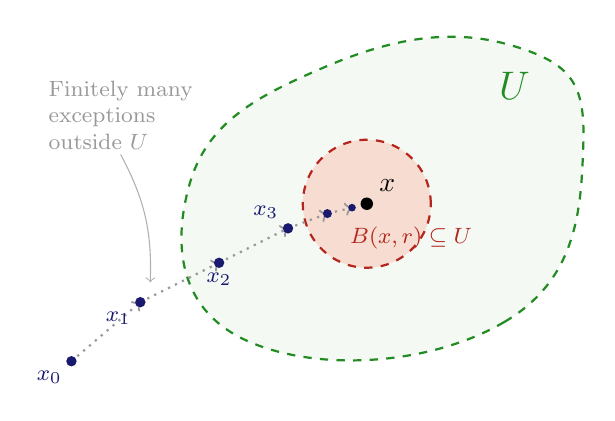
\begin{tikzpicture}[scale=1.25]
% \begin{hidden}
% - Canvas: scale=1.25, x in [-2.5, 3.5], y in [-1.5, 2.5].
% - Elements:
%   (1) Open set U: smooth dashed curve, light fill ForestGreen!5.
%   (2) Target point x in U at (1.0, 0.6).
%   (3) Open ball B(x, r): dashed circle of radius r = 0.65 centered at x, fill BrickRed!10.
%   (4) Sequence points x_n: points x_0, x_1 outside U, x_2 entering, x_3, x_4, x_5 inside B(x, r).
%   (5) Directional dashed trajectory arrows connecting x_0 -> x_1 -> ... -> x.
%   (6) Labels: U, x, B(x, r), and x_n indices.
% - Collisions: x labeled below right, B(x, r) labeled inside ball, trajectory clear of U boundary text.
% \end{hidden}

    % Open set U with dashed boundary
    \fill[ForestGreen!5] plot [smooth cycle, tension=0.8] coordinates {
        (-0.2, -0.8) (2.4, -0.6) (3.2, 1.2) (2.5, 2.2) (0.6, 2.0) (-0.8, 0.8)
    };
    \draw[thick, dashed, ForestGreen] plot [smooth cycle, tension=0.8] coordinates {
        (-0.2, -0.8) (2.4, -0.6) (3.2, 1.2) (2.5, 2.2) (0.6, 2.0) (-0.8, 0.8)
    };
    \node[ForestGreen, font=\Large\bfseries] at (2.5, 1.8) {$U$};

    % Center point x and ball B(x, r)
    \coordinate (X) at (1.0, 0.6);
    \draw[thick, dashed, BrickRed, fill=BrickRed!12] (X) circle (0.65);
    \node[BrickRed, font=\footnotesize] at (1.45, 0.25) {$B(x, r) \subseteq U$};

    % Target point x
    \fill[black] (X) circle (1.8pt) node[above right=1pt] {$x$};

    % Sequence points approaching x from outside U
    \coordinate (P0) at (-2.0, -1.0);
    \coordinate (P1) at (-1.3, -0.4);
    \coordinate (P2) at (-0.5, 0.0);
    \coordinate (P3) at (0.2, 0.35);
    \coordinate (P4) at (0.6, 0.5);
    \coordinate (P5) at (0.85, 0.56);

    \draw[->, dotted, thick, gray!80] (P0) -- (P1);
    \draw[->, dotted, thick, gray!80] (P1) -- (P2);
    \draw[->, dotted, thick, gray!80] (P2) -- (P3);
    \draw[->, dotted, thick, gray!80] (P3) -- (P4);
    \draw[->, dotted, thick, gray!80] (P4) -- (P5);

    \fill[MidnightBlue] (P0) circle (1.5pt) node[below left, font=\footnotesize] {$x_0$};
    \fill[MidnightBlue] (P1) circle (1.5pt) node[below left, font=\footnotesize] {$x_1$};
    \fill[MidnightBlue] (P2) circle (1.5pt) node[below, font=\footnotesize] {$x_2$};
    \fill[MidnightBlue] (P3) circle (1.5pt) node[above left, font=\footnotesize] {$x_3$};
    \fill[MidnightBlue] (P4) circle (1.3pt);
    \fill[MidnightBlue] (P5) circle (1.1pt);

    \node[gray!80, font=\footnotesize, align=left] at (-1.5, 1.5) {Finitely many\\exceptions\\outside $U$};
    \draw[->, gray!60, thin] (-1.5, 1.1) to[bend left=15] (-1.2, -0.2);
\end{tikzpicture}
\end{center}

\begin{steps}[Core Mechanism of the Forward Implication]
Since $U$ is open and $x \in U$, there exists an open ball $B(x, r) \subseteq U$. By definition of convergence $x_n \to x$, for this radius $r > 0$, there exists an index $N \in \mathbb{N}$ such that $x_n \in B(x, r)$ for all $n \ge N$. Since $B(x, r) \subseteq U$, it follows that $x_n \in U$ for all $n \ge N$. The only terms that can possibly lie outside $U$ belong to the finite initial set $\{x_0, x_1, \dots, x_{N-1}\}$.
\end{steps}
\end{content}

\subsection{The Notion of \texorpdfstring{\qt{Eventually}}{Eventually}}

\begin{speech}[00:38:59 - 00:39:59]
This concept of \qt{up to finitely many exceptions} is very useful, and it is very nice to say things concisely, so we give a name to this. You have a more formal definition in the notes.

When you have a sequence, and some property --- like, for instance, being in $U$ --- is true up to finitely many exceptions, we say that this property happens \emph{eventually}. \inlinemetanote{writes $\iff \text{eventually}$}

This is a word I will use many times, okay? Whenever I have a sequence and I say that this happens eventually, it means that maybe at the beginning of the sequence it is not happening, but if I wait long enough, for $n$ large enough, it will happen, and then it never stops happening. Yeah? \inlinemetanote{taps the board}
\end{speech}

\begin{student}[Student Question: Formal Meaning of \qt{Eventually}]
Is this eventually equivalent to saying there exists a big $N$ such that for all $n$ bigger than big $N$, this holds?
\end{student}

\begin{speech}[00:40:08 - 00:40:54]
Exactly. Up to finitely many exceptions means that --- if you want, this is equivalent by definition to \qt{eventually}, which is equivalent to: \inlinemetanote{writes $\iff \exists N \text{ st } \forall n \ge N$} there exists some $N$ such that for all $n \ge N$, the property holds. And this $N$ just counts how many exceptions you have; it is an upper bound for the number of exceptions.

All of these mean the same thing. You will see that it is very useful to say things concisely with this \qt{eventually}. That's why I introduced it, and it's very standard as well.
\end{speech}

\begin{content}
\begin{definition}[Eventually]\label[definition]{def:eventually}
Let $(x_n)_{n \ge 0}$ be a sequence and $P(x_n)$ a mathematical predicate. We say that $P(x_n)$ holds \newterm{eventually} (or for all $n$ up to finitely many exceptions) if:
\begin{equation}\label{eq:eventually-def}
\exists N \in \mathbb{N} \ \forall n \ge N \colon \quad P(x_n) \text{ is true}.
\end{equation}
In particular, $x_n \in U$ eventually if and only if $\exists N \in \mathbb{N}$ such that $x_n \in U$ for all $n \ge N$.
\end{definition}
\end{content}

\subsection{Sequential Characterization of Closed Sets}

\begin{speech}[00:40:54 - 00:42:14]
And the second part: \inlinemetanote{writes \qt{(2) $A \subset X$ closed $\iff$ [ whenever $(x_n)_{n \ge 0} \subset A$, $x_n \to x \implies x \in A$ ]}} A subset $A$ is closed if and only if, whenever I have a sequence contained in $A$ and the sequence converges to some limit point in $X$, then the limit belongs to $A$.

That is what I said earlier, more or less, right? Being closed.

So, here, by closed... \inlinemetanote{bell rings in the hallway, students begin talking} Well, let's take a break, yeah.
\end{speech}

\begin{content}
\begin{lemma}[Sequential Characterization of Closed Sets]\label[lemma]{lem:closed-sets-sequences}
Let $(X, d)$ be a metric space.
\begin{enumerate}[label=\textbf{(\arabic*)}]
    \setcounter{enumi}{1}
    \item \textbf{Closed Sets:} A subset $A \subseteq X$ is closed if and only if it is closed under taking limits of sequences in $A$:
    \begin{equation}\label{eq:seq-closed-def}
    A \subseteq X \text{ is closed} \iff \left[ \begin{aligned} &\text{whenever } (x_n)_{n \ge 0} \subseteq A \text{ and } x_n \to x \in X, \\ &\implies x \in A \end{aligned} \right].
    \end{equation}
\end{enumerate}
\end{lemma}

\begin{steps}[Equivalence with Sequential Closure]
Recall that the closure $\overline{A}$ was defined in \eqref{eq:closure-sequential-def} as the set of all limits of sequences in $A$. \Cref{lem:closed-sets-sequences} asserts that $A$ is closed if and only if $A = \overline{A}$, establishing complete consistency with the topological definition.
\end{steps}
\end{content}

\begin{content}[Full Statement: Sequential Characterization of Open and Closed Sets]
\begin{lemma}[Sequential Characterization of Open and Closed Sets (Complete Statement)]\label[lemma]{lem:open-closed-sequences-complete}
Let $(X, d)$ be a metric space.
\begin{enumerate}[label=\textbf{(\arabic*)}]
    \item \textbf{Open Sets:} A subset $U \subseteq X$ is open if and only if for every sequence $(x_n)_{n \ge 0} \subseteq X$ converging to a point $x \in U$, the sequence belongs to $U$ eventually:
    \begin{equation}
    U \subseteq X \text{ is open} \iff \Bigl( \forall (x_n)_{n \ge 0} \subseteq X \colon x_n \to x \in U \implies \exists N \in \mathbb{N} \ \forall n \ge N \colon x_n \in U \Bigr).
    \end{equation}
    \item \textbf{Closed Sets:} A subset $A \subseteq X$ is closed if and only if it contains all limits of sequences in $A$:
    \begin{equation}
    A \subseteq X \text{ is closed} \iff \Bigl( \forall (x_n)_{n \ge 0} \subseteq A \colon x_n \to x \in X \implies x \in A \Bigr).
    \end{equation}
\end{enumerate}
\end{lemma}
\end{content}

\subsection{Clarification on Quantifiers and Commencement of the Proof}

\begin{speech}[00:42:14 - 00:43:04]
\inlinemetanote{classroom noise and chatter as students talk loudly} Please... Please... Okay, I will start if you don't listen... \inlinemetanote{laughter}

May you forgive me for the stereotype, but when I studied mathematics in Barcelona --- which is a Mediterranean country --- people started the lecture on time, so they were silent. We are in Switzerland: you should be like the champions of starting on time! And I'm seeing the contrary; I'm very surprised. Okay. \inlinemetanote{wipes the lower right chalkboard with a sponge}

And you know this is recorded, so the proof of the misbehavior will be there for history. Okay.
\end{speech}

\begin{speech}[00:43:05 - 00:43:55]
We said we are going to prove \textbf{(1)}.

So, I said that $U$ open is equivalent to this property. Let me clarify, because this is a terminology that is very useful, but maybe you are not familiar with it: when I say \qt{whenever}, it means whenever. That is, for all sequences... \inlinemetanote{writes $\forall \text{ seq}$ above \qt{whenever}} For every sequence satisfying this, then that happens, right? \qt{Whenever} is like a \qt{for all}.

So, \qt{whenever} essentially means \qt{for all}.
\end{speech}

\begin{content}[Logical Parsing of the Statement]
In the formulation of \cref{lem:open-closed-sequences}:
\[
\text{\qt{whenever }} (x_n)_{n \ge 0} \subseteq X \text{ with } x_n \to x \in U \implies x_n \in U \text{ eventually}
\]
the term \qt{whenever} is a formal universal quantifier over all sequences in $X$:
\[
\forall (x_n)_{n \ge 0} \subseteq X \colon \quad \bigl( x_n \to x \text{ with } x \in U \implies \exists N \in \mathbb{N} \ \forall n \ge N \colon x_n \in U \bigr).
\]
\end{content}

\subsection{Proof of the Sequential Characterization of Open Sets}

\begin{proofWrapper}[Proof of Lemma \ref{lem:open-closed-sequences}, Part (1)]

\subsubsection{Forward Implication (\texorpdfstring{$\implies$}{=>})}

\begin{speech}[00:43:55 - 00:45:06]
Proof of \textbf{(1)}. \inlinemetanote{writes \qt{proof (1) $\implies$} on the lower right chalkboard} I need to do two implications. First, I will do this direction, which is the one I've been drawing here.

Assume that $U$ is open. Now, I'm just going to put in symbols the drawing that I did here. Take $x \in U$ \inlinemetanote{writes \qt{take $x \in U$}}, any point. By definition of an open set, since $U$ is open, there exists some $r > 0$ such that the ball of radius $r$ centered at $x$ is contained in $U$, right? \inlinemetanote{writes $\implies \exists r > 0 \text{ st } B(x, r) \subset U$ and notes \qt{given $U$ open}}
\end{speech}

\begin{content}[Forward Implication: Openness Implies Eventual Containment]
\textbf{Goal ($\implies$):} Assume $U \subseteq X$ is open. Let $(x_n)_{n \ge 0} \subseteq X$ be any sequence converging to a point $x \in U$. We must show that $x_n \in U$ eventually.

\par\vspace{1ex}\noindent
Let $x \in U$. Since $U$ is open by assumption, there exists a radius $r > 0$ such that:
\begin{equation}\label{eq:ball-inside-U}
B(x, r) \subseteq U.
\end{equation}
\end{content}

\begin{speech}[00:45:06 - 00:46:58]
And now, since by assumption $x_n$ converges to $x$ \inlinemetanote{writes \qt{Since $x_n \to x$}}... What was the definition of convergence? Remember: given any $\varepsilon$ --- in the definition I called this $\varepsilon$ \inlinemetanote{points at $r > 0$}, right? Given any $\varepsilon$, now it is $r$, but it is the same --- for $n$ large enough, bigger than a certain capital $N$, my sequence will belong to the ball of radius $r$.

So, since $x_n$ converges to $x$, there exists some capital $N$, depending on $r$, such that \inlinemetanote{writes $\exists N \text{ st }$} $x_n$ belongs to the ball of radius $r$ centered at $x$ for all $n \ge N$: \inlinemetanote{writes $x_n \in B(x, r) \ \forall n \ge N$}

Now, in the definition of convergence, maybe there was not this ball, but there was something equivalent: distance. This is the same: saying that $x_n \in B(x, r)$ is the same as saying that the distance between $x_n$ and $x$ is less than $r$. \inlinemetanote{boxes $x_n \in B(x, r)$ and writes $\iff d(x_n, x) < r$} Because when does a point belong to the ball? When the distance to the center is strictly less than $r$. This is if and only if, right?

And this is what I'm saying here: end of the proof. \inlinemetanote{draws $\square$} Because up to finitely many exceptions --- that is this capital $N$ --- all subsequent points of the sequence belong to the ball, and the ball is contained in $U$, so they belong to $U$, right? So, this proves this implication.
\end{speech}

\begin{content}[Conclusion of Forward Implication]
Since $x_n \to x$, by the definition of convergence with $\varepsilon = r > 0$, there exists an index threshold $N = N(r) \in \mathbb{N}$ such that:
\begin{equation}\label{eq:convergence-radius-r}
d(x_n, x) < r \quad \forall n \ge N.
\end{equation}
By definition of the open ball, this condition is identical to:
\begin{equation}\label{eq:points-in-ball}
x_n \in B(x, r) \quad \forall n \ge N.
\end{equation}
Since $B(x, r) \subseteq U$ from \eqref{eq:ball-inside-U}, we conclude:
\[
x_n \in U \quad \forall n \ge N.
\]
Thus, $x_n \in U$ eventually (for all $n$ up to finitely many exceptions). This completes the proof of the forward implication $\implies$.
\end{content}

\begin{hidden}
% timestamp: 00:07:00
% topic: Completed forward implication (U open => seq converges inside U eventually)
% board_state: eq:ball-inside-U, eq:convergence-radius-r, eq:points-in-ball
% next_goal: Prove reverse implication (<=) by contraposition: not open => exists sequence escaping U
% open_loops: none
\end{hidden}

\subsubsection{Reverse Implication (\texorpdfstring{$\Leftarrow$}{<=}) by Contraposition}

\begin{speech}[00:46:58 - 00:48:45]
Now, still for \textbf{(1)}, I will prove the second implication --- the one this way: \inlinemetanote{writes $\Leftarrow$ in a box}

And I will prove this by contraposition, right? $A \implies B$ is equivalent to $\neg B \implies \neg A$, right? We know that. To prove this, I will prove that not-left gives not-right: \inlinemetanote{writes $\neg \text{left} \implies \neg \text{right}$ and \qt{contraposition}} This is a proof by contraposition.

Now, let's do a bit of logic. What is the negation of $U$ open? Remember the definition of $U$ open: for every point in my set $U$, there exists some radius such that the ball is contained in $U$, right?

And now we take the negation. The negation of \qt{for every point} is \qt{there exists a point}. So, the negation --- $U$ is not open --- is the same as: there exists $x \in U$ \inlinemetanote{writes \qt{$U$ not open $\iff \exists x \in U$}} such that for every radius $r > 0$ \inlinemetanote{writes $\forall r > 0$}, the ball centered at $x$ with radius $r$ is not contained in $U$: \inlinemetanote{writes $B(x, r) \not\subset U$}
\end{speech}

\begin{content}[Logical Setup of Contraposition]
\textbf{Goal ($\Leftarrow$):} We wish to prove:
\[
\bigl( \text{whenever } x_n \to x \in U \implies x_n \in U \text{ eventually} \bigr) \implies U \text{ is open}.
\]
We prove this by contraposition ($\neg \text{left} \implies \neg \text{right}$):
\[
U \text{ is not open} \implies \neg \bigl( \forall (x_n) \subseteq X \colon x_n \to x \in U \implies x_n \in U \text{ eventually} \bigr).
\]

\textbf{Negating Openness:}
Recall the definition of openness:
\[
U \text{ is open} \iff \forall x \in U \ \exists r > 0 \colon B(x, r) \subseteq U.
\]
Negating this statement yields:
\begin{align}
U \text{ is not open} &\iff \neg \bigl( \forall x \in U \ \exists r > 0 \colon B(x, r) \subseteq U \bigr) \nonumber \\
&\iff \exists x \in U \ \forall r > 0 \colon B(x, r) \not\subseteq U. \label{eq:negation-openness}
\end{align}
\end{content}

\begin{speech}[00:48:45 - 00:50:46]
And that the ball is not contained in $U$ is the same as saying that there exists some point --- let's call it $x_r$, because it depends on $r$ --- that belongs to the complement: \inlinemetanote{writes $\iff \exists x_r \in B(x, r) \cap (X \setminus U)$}

What am I saying here? Now I will do a drawing of that.

I take a set that is not open --- let me call it $E$: \inlinemetanote{draws a sketch of set $E$ on the middle-left chalkboard with a solid boundary segment} Heuristically, if the skin were not contained, it would be open. I draw it like this because there is a piece of skin, so it is not open, okay? This is just to make the drawing.

Now, I'm saying: there exists a point $x$ on the skin \inlinemetanote{marks $x$ on the solid boundary of $E$ } such that for every radius that I choose here, I can find a point outside my set. This point is what I called $x_r$, right? \inlinemetanote{marks $x_r$ outside $E$ in the circle around $x$} In other words, there is some point in the set that can be approximated by a sequence of points from outside the set.
\end{speech}

\begin{content}[Geometric Construction of Approximating Sequence]
The condition $B(x, r) \not\subseteq U$ means that for every $r > 0$, the ball contains at least one point outside $U$:
\begin{equation}\label{eq:point-outside-U}
B(x, r) \not\subseteq U \iff \exists x_r \in B(x, r) \cap (X \setminus U).
\end{equation}

\begin{center}
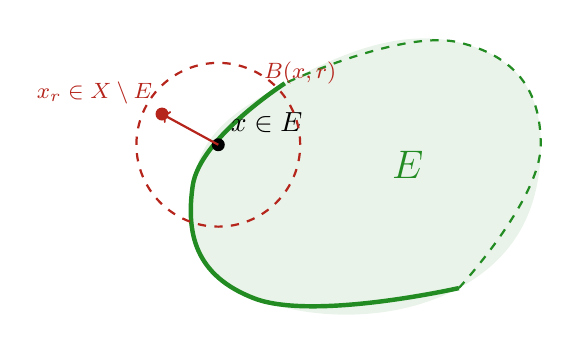
\begin{tikzpicture}[scale=1.3]
% \begin{hidden}
% - Canvas: scale 1.3, x-range [-1.5, 3.5], y-range [-1.5, 2.5]
% - Elements: (1) non-open set E with dashed and solid boundary sections; (2) point x on the solid boundary;
%   (3) dashed ball B(x, r); (4) point x_r outside E inside the ball
% - Coordinates: x at (-0.35, 1.0); ball radius r = 0.8; point x_r at (-0.9, 1.3) outside E
% - Labels: E inside the set, x on the boundary, x_r in the complement, B(x, r) near the ball
% - Collisions: labels spatially separated, no overlap
% \end{hidden}
    % Domain E (non-open set with a piece of boundary included)
    \fill[ForestGreen!10] plot [smooth cycle, tension=0.8] coordinates {
        (0, -0.5) (2.0, -0.4) (2.8, 1.0) (2.0, 2.0) (0.3, 1.6) (-0.6, 0.6)
    };

    % Dashed part of boundary (excluded skin)
    \draw[thick, dashed, ForestGreen] plot [smooth, tension=0.8] coordinates {
        (2.0, -0.4) (2.8, 1.0) (2.0, 2.0) (0.3, 1.6)
    };
    % Solid part of boundary (included skin, making the set not open)
    \draw[ultra thick, ForestGreen] plot [smooth, tension=0.8] coordinates {
        (0.3, 1.6) (-0.6, 0.6) (0, -0.5) (2.0, -0.4)
    };

    \node[ForestGreen, font=\Large\bfseries] at (1.5, 0.8) {$E$};

    % Point x on the included boundary
    \coordinate (X) at (-0.35, 1.0);
    \fill[black] (X) circle (1.8pt) node[above right=1pt] {$x \in E$};

    % Ball B(x, r) around x
    \draw[thick, dashed, BrickRed] (X) circle (0.8);
    \node[BrickRed, font=\footnotesize] at (0.45, 1.7) {$B(x, r)$};

    % Point x_r in B(x, r) \setminus E
    \coordinate (XR) at (-0.9, 1.3);
    \fill[BrickRed] (XR) circle (1.8pt) node[above left, text=BrickRed, font=\footnotesize] {$x_r \in X \setminus E$};
    \draw[->, thick, BrickRed] (X) -- (XR);
\end{tikzpicture}
\end{center}

\begin{steps}[Heuristic Idea: Approximating a Boundary Point from Outside]
If $E$ contains a portion of its boundary (\qt{skin}), any point $x$ on this boundary cannot be insulated by an open ball. Every ball $B(x, r)$, no matter how small, must leak into the exterior $X \setminus E$, providing an escape point $x_r \notin E$.
\end{steps}
\end{content}

\begin{speech}[00:50:46 - 00:52:28]
Taking $r = 1/n$ for $n \ge 1$ \inlinemetanote{writes \qt{taking $r = 1/n, n \ge 1$}}, I produce a sequence of points. These balls are smaller and smaller, and these points $x_r$ --- I define $x_n := x_{r=1/n}$ \inlinemetanote{writes $x_n := x_{r=1/n}$}. These points are in balls closer and closer to $x$, so they converge to the point $x$, right? \inlinemetanote{writes $x_n \to x$}

I found a sequence that converges to the point $x$, and that comes from the outside.

But then, this is false. Because the statement says that up to finitely many exceptions, the sequence should be contained in $U$, whereas all the elements of this sequence are outside of $U$! So, this contradicts that $x_n$ belongs to $U$ eventually: \inlinemetanote{writes \qt{contradicts $x_n \in U$ eventually}}

This contradicts that $x_n \in U$ eventually, and that ends the proof of this implication. \inlinemetanote{draws $\square$}

I proved that not-left implies not-right, right? Except for the spelling. \inlinemetanote{laughter}
\end{speech}

\begin{content}[Contradiction and Conclusion of Reverse Implication]
We now construct an explicit escaping sequence. For each $n \in \mathbb{N}_{\ge 1}$, we choose the radius:
\begin{equation}\label{eq:radius-1-over-n}
r_n := \frac{1}{n} > 0.
\end{equation}
By \eqref{eq:point-outside-U}, for each $n \ge 1$ there exists a point $x_n := x_{1/n}$ such that:
\begin{equation}\label{eq:escaping-sequence-def}
x_n \in B\left( x, \frac{1}{n} \right) \cap (X \setminus U).
\end{equation}
Because $x_n \in B(x, 1/n)$, the distance satisfies:
\[
d(x_n, x) < \frac{1}{n} \xrightarrow{n \to \infty} 0,
\]
which proves that $x_n \to x \in U$.

\par\vspace{1ex}\noindent
However, by construction, every term of the sequence lies in the complement of $U$:
\[
x_n \in X \setminus U \iff x_n \notin U \quad \forall n \ge 1.
\]
Therefore, $x_n$ can never belong to $U$, which directly contradicts the assertion that $x_n \in U$ eventually!

\par\vspace{1ex}\noindent
Thus, assuming $U$ is not open implies the existence of a sequence $x_n \to x \in U$ that is not eventually in $U$. By contraposition, this completes the proof of the reverse implication $\Leftarrow$.
\end{content}

\end{proofWrapper}

\begin{hidden}
% timestamp: 00:12:30
% topic: Completed proof of Lemma 1 (open sets through sequences).
% board_state: lem:open-closed-sequences, eq:escaping-sequence-def
% next_goal: Address student questions, leave part (2) as exercise, move to continuity
% open_loops: none
\end{hidden}

\subsection{Student Interaction: Notation of Subset Symbols}

\begin{speech}[00:52:28 - 00:53:26]
Is this okay, this type of proof?

This is the usual problem when I see people who look very serious: I don't know if they are completely lost, if they find it super boring, or what the problem is. So, if someone has questions and wants to participate, we can slow down and ask questions. Otherwise, we continue with other stuff.

We still need to do this one, right? \inlinemetanote{points at Part \textbf{(2)} of the Lemma on the left board} Good.

Ah, there is a question... Sorry? Up there, I don't see? Ah, there! Oh, nice. Thank you. \inlinemetanote{tosses catch-box microphone up to student}
\end{speech}

\begin{student}[Student Question: Notation for Subsets]
You write the... you write the subset symbol without the equality sign at the bottom. Does it have a meaning, or like that it cannot be equal, or is that just notation? Like, subset without the extra line at the bottom.
\end{student}

\begin{speech}[00:53:38 - 00:54:06]
Ah, you mean this? \inlinemetanote{points to $\subset$ on the board} It's the same. You mean this? \inlinemetanote{points to $\subset$ again} Well, it's not the same symbol, but it's the same meaning.

Some people use the equality line. Since it means the same, I save one line, right? But this is very standard; many people just use this. So, I will always use this \qt{contained} symbol without the equality sign.
\end{speech}

\begin{content}
\begin{remark}[Standing Convention: Subset Notation $\subset$ vs. $\subseteq$]\label[remark]{rem:subset-notation}
Throughout this course, the symbol $\subset$ is used interchangeably with $\subseteq$ to denote non-strict set inclusion:
\[
A \subset B \iff A \subseteq B \iff \forall x \in A \colon x \in B.
\]
In particular, $A \subset B$ permits the possibility that $A = B$. If a strict (proper) subset is intended, it will be stated explicitly.
\end{remark}
\end{content}

\subsection{Exercises: Sequential Closedness and Metric Subspaces}

\begin{speech}[00:54:06 - 00:55:23]
Any others? Thanks. \inlinemetanote{catches microphone back}

Let's do this, because maybe you will find continuous functions more exciting. Since this proof over here is super similar to the previous one --- and again, you see that these proofs are one-line proofs, just using the definitions and manipulating them around --- I leave this proof as an exercise. Try to do it. If you understood the definitions well and can draw a picture of what's going on, this shouldn't be too difficult.

It can be a bit difficult at the beginning because there are a lot of new definitions and you need to learn them. But the best way is to practice with these exercises and try to do them by yourself. Because if I do them, it looks like a bunch of symbols that all work out, but you don't internalize the definitions. The best way is to try by yourself.
\end{speech}

\begin{content}
\begin{exercise}[Sequential Characterization of Closed Sets]\label[exercise]{ex:seq-closed-proof}
Prove Part \textbf{(2)} of \cref{lem:open-closed-sequences}: Let $(X, d)$ be a metric space. A subset $A \subseteq X$ is closed if and only if:
\[
\text{whenever } (x_n)_{n \ge 0} \subseteq A \text{ and } x_n \to x \in X \implies x \in A.
\]
\end{exercise}

\begin{steps}[Proof Strategy for the Exercise]
\begin{itemize}
    \item \textbf{Direction $\implies$:} Assume $A$ is closed, so $X \setminus A$ is open. If $(x_n) \subseteq A$ converges to $x \in X \setminus A$, then by Part \textbf{(1)}, $x_n \in X \setminus A$ eventually, contradicting that all $x_n \in A$. Hence, $x \in A$.
    \item \textbf{Direction $\Leftarrow$:} Assume $A$ is sequentially closed. To show $X \setminus A$ is open, apply Part \textbf{(1)}: if $x_n \to x \in X \setminus A$ but $x_n \in A$ for infinitely many $n$, a subsequence in $A$ converges to $x \in A$, a contradiction.
\end{itemize}
\end{steps}
\end{content}

\begin{speech}[00:55:23 - 00:56:54]
Now I will do something more exciting, which is continuity. Or maybe I can put another exercise --- you have more in the exercise list: \inlinemetanote{writes \qt{exercise} on the board}

Exercise before continuity: Now that you have all of this, you can prove that if $(X, d)$ is a complete metric space \inlinemetanote{writes $(X, d) \text{ complete}$} and $A \subset X$ is a closed subset \inlinemetanote{writes $A \subset X \text{ closed}$}, then $A$ with the same distance restricted is complete: \inlinemetanote{writes $(A, d) \text{ complete}$}

Example: we know that $\mathbb{R}^n$ is a complete metric space. Then any closed subset of $\mathbb{R}^n$ will be a complete metric space when you restrict the distance.

Now you have all the ingredients to prove that. It's not too difficult; it's a good exercise.
\end{speech}

\begin{content}
\begin{exercise}[Closed Subsets of Complete Metric Spaces Are Complete]\label[exercise]{ex:closed-subsets-complete}
Let $(X, d)$ be a complete metric space and $A \subseteq X$ a closed subset. Prove that the subspace $(A, d|_{A \times A})$ is a complete metric space.
\end{exercise}

\begin{example}[Complete Subspaces of $\mathbb{R}^n$]\label[example]{ex:rn-closed-subspaces-complete}
Since $(\mathbb{R}^n, d_{\text{Euc}})$ is complete, every closed subset $A \subseteq \mathbb{R}^n$ (such as closed balls, closed cubes, or submanifolds without boundary) equipped with the Euclidean distance is a complete metric space.
\end{example}

\begin{steps}[Guided Derivation for \cref{ex:closed-subsets-complete}]
\begin{enumerate}[label=\textbf{(\arabic*)}]
    \item Let $(x_n)_{n \ge 0} \subseteq A$ be a Cauchy sequence in $(A, d|_{A \times A})$.
    \item Since the metric on $A$ is the restriction of $d$, $(x_n)_{n \ge 0}$ is also a Cauchy sequence in the ambient space $(X, d)$.
    \item Since $(X, d)$ is complete, there exists a limit $x \in X$ such that $x_n \to x$ in $(X, d)$.
    \item Because $A$ is closed, by \cref{lem:closed-sets-sequences} the limit point must lie in $A$ ($x \in A$).
    \item Thus, the Cauchy sequence converges to a limit inside $A$, proving that $(A, d|_{A \times A})$ is complete.
\end{enumerate}
\end{steps}
\end{content}

\section{Continuity in Metric Spaces}

\subsection{Definition of Continuous Maps Between Metric Spaces}

\begin{speech}[00:56:54 - 00:58:23]
I will switch to something that is a bit more fun, which is continuity, because you already know...

Now we start to have problems with the shadows. Someone --- I don't remember who --- complained about shadows. Now I can write here, right? It's just when the other blackboard is annoying, okay.

Now we'll see continuity. \inlinemetanote{writes \qt{Continuity} as header on the left board} For continuity, we will define continuous maps. We will be in this setup: $f$ will be a map between two sets $X$ and $Y$ \inlinemetanote{writes $f \colon X \to Y$}, and they are both metric spaces. So, we will have $X$ with its distance $d_X$, and $Y$ with its distance $d_Y$: \inlinemetanote{writes $(X, d_X), (Y, d_Y) \text{ metric spaces}$}
\end{speech}

\begin{content}[Setup for Continuity]
\textbf{Setting for Continuous Mappings:}
Let $(X, d_X)$ and $(Y, d_Y)$ be two metric spaces, and let:
\[
f \colon X \to Y
\]
be a mapping from $X$ into $Y$.
\end{content}

\begin{speech}[00:58:23 - 00:59:43]
Many times for us, these sets will be the Euclidean space of some dimension and the Euclidean space of some other dimension, right? But they can be whatever. Both are metric spaces --- different or the same.

Now, the definition: \inlinemetanote{writes \qt{Def'n}} We say that a map $f$ is continuous \inlinemetanote{writes \qt{$f$ is continuous}} if one of the following three equivalent properties holds true: \inlinemetanote{writes \qt{if one of the following 3 equivalent properties hold true:}}

I will state the three definitions of continuity, because you are already very familiar with at least two of them from Analysis~I, right? But I will state them now by postulating that they are equivalent, and later we will prove immediately that they are indeed equivalent, right?
\end{speech}

\begin{content}
\begin{definition}[Continuous Mapping between Metric Spaces]\label[definition]{def:continuity-metric-spaces}
Let $(X, d_X)$ and $(Y, d_Y)$ be metric spaces. A mapping $f \colon X \to Y$ is called \newterm{continuous} if any one of the following three equivalent properties holds true:
\begin{enumerate}[label=\textbf{(\arabic*)}]
    \item \textbf{$\varepsilon$-$\delta$ Continuity (Local/Metric Form):} For every point $x \in X$, small variations in $x$ produce arbitrarily small variations in $f(x)$.
    \item \textbf{Sequential Continuity:} $f$ preserves convergent sequences: whenever $x_n \to x$ in $X$, then $f(x_n) \to f(x)$ in $Y$.
    \item \textbf{Topological Continuity (Pre-images of Open Sets):} For every open subset $V \subseteq Y$, the pre-image $f^{-1}(V)$ is open in $X$.
\end{enumerate}
\end{definition}
\end{content}

\begin{hidden}
% timestamp: 00:18:30
% topic: Setup for continuous mappings between metric spaces (X, d_X) and (Y, d_Y).
% board_state: def:continuity-metric-spaces
% next_goal: Formulate definition (1): epsilon-delta continuity and ball reformulation.
% open_loops: none
\end{hidden}

\subsection{Definition (1): \texorpdfstring{$\varepsilon$-$\delta$}{Epsilon-Delta} Continuity}

\begin{speech}[00:59:43 - 01:00:23]
Definition \textbf{(1)} of continuity is the $\varepsilon$-$\delta$ continuity that you are familiar with. \inlinemetanote{writes \qt{(1) $\varepsilon$-$\delta$} in a box}

You know this very well for functions of one real variable. Now we need to abstract the same notion to metric spaces. How was the definition with $\varepsilon$-$\delta$? Can someone remind me: on the real line, what is the definition of continuity with $\varepsilon$-$\delta$? Does someone remember? \inlinemetanote{holds up catch-box microphone and looks at the class}

Yeah, good. \inlinemetanote{throws microphone to student}
\end{speech}

\begin{student}[Student Answer: Definition of $\varepsilon$-$\delta$ Continuity]
Hello? Hello. Is it working? Okay, so I think it was... a function is continuous at $x_0$ if for every $\varepsilon$ larger than zero, there exists a $\delta$ such that for all $x$ minus, that's $x - x_0$ smaller than $\delta$, $f(x) - f(x_0)$ is smaller than $\varepsilon$, and if that holds, yeah.
\end{student}

\begin{speech}[01:00:52 - 01:02:43]
Up to here is very good. You said what is continuous at a point. For a continuous function, it is continuous at all points --- you were going to say that. But I will use directly continuous at every point.

I will start exactly as you said. First I will add --- since I want it to be continuous at every point --- \qt{for every point, for all $x \in X$}: \inlinemetanote{writes $\forall x \in X$}

Next is what you said: for every $x$, given --- \qt{given} is \qt{for all $\varepsilon > 0$} --- there exists $\delta > 0$: \inlinemetanote{writes $\forall \varepsilon > 0 \ \exists \delta > 0$}

And now the rest of your definition used intervals and stuff that are not available in metric spaces, so how do we translate? The notion will be that if the distance between $x$ and $x'$ is less than $\delta$, then the distance between $f(x)$ and $f(x')$ is less than $\varepsilon$: \inlinemetanote{writes $[ d(x, x') < \delta \implies d(f(x), f(x')) < \varepsilon ]$}

And what is this distance? This distance is the distance in the space here, $X$, and these guys belong to $Y$, so this is the distance in $Y$. \inlinemetanote{adds subscripts $d_X$ and $d_Y$} Right? What else could it be? It cannot be anything else. If you think about this, it's the only way to generalize.

Another way to say this: for all $x' \in X$ that satisfies this, it also satisfies that, okay? \inlinemetanote{writes $(\forall x' \in X)$ above}
\end{speech}

\begin{content}
\begin{definition}[$\varepsilon$-$\delta$ Continuity]\label[definition]{def:eps-delta-continuity}
Let $(X, d_X)$ and $(Y, d_Y)$ be metric spaces. A map $f \colon X \to Y$ is \newterm{$\varepsilon$-$\delta$ continuous} if for every point $x \in X$ and every tolerance $\varepsilon > 0$, there exists a radius $\delta > 0$ such that all points within distance $\delta$ from $x$ map to points within distance $\varepsilon$ from $f(x)$:
\begin{equation}\label{eq:eps-delta-def}
\forall x \in X \ \forall \varepsilon > 0 \ \exists \delta > 0 \colon \quad \Bigl[ \forall x' \in X \colon d_X(x, x') < \delta \implies d_Y(f(x), f(x')) < \varepsilon \Bigr].
\end{equation}
\end{definition}

\begin{steps}[From $\mathbb{R}$ to Metric Spaces]
In standard real analysis on $\mathbb{R}$, distance is measured via the absolute value $|x - x'| < \delta$ and $|f(x) - f(x')| < \varepsilon$. In arbitrary metric spaces, these absolute values are replaced by the corresponding metric distance functions $d_X(x, x')$ and $d_Y(f(x), f(x'))$.
\end{steps}
\end{content}

\subsection{Reformulation via Open Balls}

\begin{speech}[01:02:43 - 01:03:44]
Another way to say this --- because this is a bit annoying to write, it's a bit long --- is to say that this thing here, the red bracket, is exactly the same as saying that when I compute $f$, the image of the ball of radius $\delta$ centered at $x$ will be contained in the ball of radius $\varepsilon$ centered at $f(x)$: \inlinemetanote{writes in red chalk $\iff [ f(B_\delta(x)) \subset B_\varepsilon(f(x)) ]$}
\end{speech}

\begin{speech}[01:03:44 - 01:04:19]
You see this? What does $f$ of this ball mean? $f$ of the ball is the image of all the points in the ball. And I'm saying that for every point in the ball of radius $\delta$ here, the image will be here, in the other ball, right?

This thing is a compact way of writing that condition, and I will use this bottom part.

So, this is the $\varepsilon$-$\delta$ definition.
\end{speech}

\begin{content}[Reformulation of Continuity via Open Balls]
The bracketed implication in \eqref{eq:eps-delta-def} can be formulated compactly using open balls:
\begin{equation}\label{eq:ball-containment-def}
\forall x' \in X \colon \Bigl( d_X(x, x') < \delta \implies d_Y(f(x), f(x')) < \varepsilon \Bigr) \iff f\bigl(B_\delta(x)\bigr) \subseteq B_\varepsilon\bigl(f(x)\bigr).
\end{equation}
Thus, the condition of $\varepsilon$-$\delta$ continuity becomes:
\begin{equation}\label{eq:continuity-ball-form}
\forall x \in X \ \forall \varepsilon > 0 \ \exists \delta > 0 \colon \quad f\bigl(B_\delta(x)\bigr) \subseteq B_\varepsilon\bigl(f(x)\bigr).
\end{equation}

\begin{center}
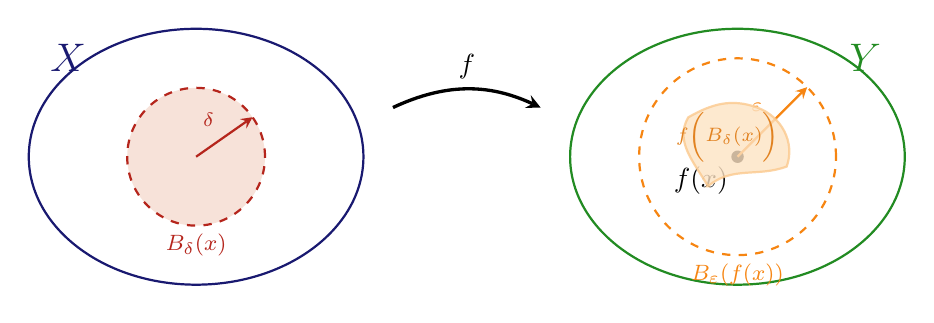
\begin{tikzpicture}[scale=1.25, >=stealth]
% \begin{hidden}
% - Canvas: scale 1.25, two metric spaces (X on left, Y on right); x-range [-2.5, 7.5], y-range [-1.8, 1.8]
% - Order: (1) metric space domains X and Y (MidnightBlue and ForestGreen ellipses); (2) center points x and f(x);
%   (3) dashed delta-ball B_delta(x) in X and dashed epsilon-ball B_epsilon(f(x)) in Y;
%   (4) shaded image f(B_delta(x)) strictly inside B_epsilon(f(x)); (5) mapping arrow f
% - Coordinates: X centered at (-0.5, 0), Y centered at (5.0, 0); x at (-0.5, 0), delta = 0.7;
%   f(x) at (5.0, 0), epsilon = 1.0; image f(B_delta(x)) filled in BurntOrange!20 inside B_epsilon(f(x))
% - Labels: clearly positioned without collisions
% \end{hidden}
    % Space X
    \draw[thick, MidnightBlue] (-0.5, 0) ellipse (1.7 and 1.3);
    \node[MidnightBlue, font=\Large\bfseries] at (-1.8, 1.0) {$X$};

    % Center point x and ball B_delta(x) in X
    \coordinate (X) at (-0.5, 0);
    \fill[black] (X) circle (1.8pt) node[below left] {$x$};
    \draw[thick, dashed, BrickRed, fill=BrickRed!10] (X) circle (0.7);
    \draw[->, thick, BrickRed] (X) -- ++(35:0.7) node[midway, above left, font=\scriptsize] {$\delta$};
    \node[BrickRed, font=\footnotesize] at (-0.5, -0.9) {$B_\delta(x)$};

    % Space Y
    \draw[thick, ForestGreen] (5.0, 0) ellipse (1.7 and 1.3);
    \node[ForestGreen, font=\Large\bfseries] at (6.3, 1.0) {$Y$};

    % Center point f(x) and ball B_epsilon(f(x)) in Y
    \coordinate (FX) at (5.0, 0);
    \fill[black] (FX) circle (1.8pt) node[below left] {$f(x)$};
    \draw[thick, dashed, BurntOrange] (FX) circle (1.0);
    \draw[->, thick, BurntOrange] (FX) -- ++(45:1.0) node[midway, above left, font=\scriptsize] {$\varepsilon$};
    \node[BurntOrange, font=\footnotesize] at (5.0, -1.2) {$B_\varepsilon(f(x))$};

    % Image f(B_delta(x)) strictly contained inside B_epsilon(f(x))
    \filldraw[thick, BurntOrange!40, fill=BurntOrange!20, opacity=0.8]
        (4.7, -0.3) to[out=40, in=200] (5.5, -0.1)
                    to[out=70, in=-20] (5.2, 0.5)
                    to[out=160, in=30] (4.5, 0.4)
                    to[out=-120, in=120] cycle;
    \node[BurntOrange!90!black, font=\scriptsize\bfseries] at (4.9, 0.2) {$f\bigl(B_\delta(x)\bigr)$};

    % Mapping arrow f between spaces
    \draw[->, very thick] (1.5, 0.5) to[bend left=25] node[midway, above] {$f$} (3.0, 0.5);
\end{tikzpicture}
\end{center}

\begin{steps}[Geometric Interpretation of Ball Containment]
The condition $f(B_\delta(x)) \subseteq B_\varepsilon(f(x))$ encapsulates the geometric essence of continuity: the mapping $f$ contracts a sufficiently small neighborhood $B_\delta(x)$ in the domain into the prescribed target tolerance ball $B_\varepsilon(f(x))$ in the codomain.
\end{steps}
\end{content}

\subsection{Definition (2): Sequential Continuity}

\begin{speech}[01:04:19 - 01:05:40]
The second definition is with sequences, right? Continuity with sequences. \inlinemetanote{writes \qt{\textbf{(2)}}}

This is essentially the same as in $\mathbb{R}$. If $(x_n)$ is a sequence converging to a point $x$, then the sequence of images, $(f(x_n))_{n \ge 0}$, is convergent \inlinemetanote{writes $(x_n)_{n \ge 0} \subset X \ \& \ x_n \to x \implies (f(x_n))_{n \ge 0}$} in the space $Y$ with limit $f(x)$. \inlinemetanote{writes \qt{is convergent in $Y$ with limit $f(x)$}}
\end{speech}

\begin{speech}[01:05:40 - 01:06:11]
A compact way to write this, if you want, is that $f(x_n)$ converges as $n \to \infty$ to $f(x)$: \inlinemetanote{writes $\iff [ f(x_n) \xrightarrow{n \to \infty} f(x) ]$}

For this, you essentially don't even need anything new: it's really the same definition as in $\mathbb{R}$; you plug it in here and it makes sense.
\end{speech}

\begin{hidden}
% timestamp: 00:06:14
% topic: Definitions of continuity in metric spaces (epsilon-delta and sequential)
% board_state: def:eps-delta-continuity, def:sequential-continuity
% next_goal: Introduce definition (3): topological continuity via open set pre-images
% open_loops: none
\end{hidden}

\begin{content}
\begin{definition}[Sequential Continuity]\label[definition]{def:sequential-continuity}
Let $(X, d_X)$ and $(Y, d_Y)$ be metric spaces. A mapping $f \colon X \to Y$ is called \newterm{sequentially continuous} if it preserves limits of convergent sequences:
\begin{equation}\label{eq:sequential-continuity-def}
\forall (x_n)_{n \ge 0} \subseteq X \text{ with } x_n \xrightarrow{n \to \infty} x \text{ in } X \implies f(x_n) \xrightarrow{n \to \infty} f(x) \text{ in } Y.
\end{equation}
\end{definition}

\begin{steps}[Sequential Preservation]
Sequential continuity states that the operations of applying the function $f$ and taking sequential limits commute:
\[
\lim_{n \to \infty} f(x_n) = f\left( \lim_{n \to \infty} x_n \right).
\]
\end{steps}
\end{content}

\subsection{Definition (3): Topological Continuity}

\begin{speech}[01:06:11 - 01:07:32]
And then there is a new... \inlinemetanote{a student sneezes: \qt{bless you}} ...a new notion of continuity, which is the topological notion of continuity. Number \textbf{(3)}: this one is new, but it will be very easy to prove that it is the same. \inlinemetanote{moves to the chalkboard on the right and writes \qt{\textbf{(3)}}}

We will use this all the time, which is why I am giving it. Topological: \inlinemetanote{writes \qt{topological}} it says that for every open $V \subset Y$ \inlinemetanote{writes $\forall V \subset Y \text{ open}$}, the preimage $f^{-1}(V)$ \inlinemetanote{writes $f^{-1}(V)$}, which is a subset of $X$ \inlinemetanote{writes $\subset X$}, is open. \inlinemetanote{writes \qt{open}}

This is the third definition of continuity. A map, a function is continuous whenever you take an open set in the target, and you look back at it --- you take $f^{-1}$ --- you get an open set here in the domain.
\end{speech}

\begin{content}
\begin{definition}[Topological Continuity]\label[definition]{def:topological-continuity}
Let $(X, d_X)$ and $(Y, d_Y)$ be metric spaces. A mapping $f \colon X \to Y$ is called \newterm{topologically continuous} if the pre-image of every open subset of $Y$ is open in $X$:
\begin{equation}\label{eq:topological-continuity-def}
\forall V \subseteq Y \text{ open in } (Y, d_Y) \implies f^{-1}(V) \subseteq X \text{ is open in } (X, d_X).
\end{equation}
\end{definition}

\begin{steps}[Pre-images vs. Forward Images]
A crucial asymmetry in topology is that continuity is defined via \textbf{pre-images} ($f^{-1}(V)$), not forward images ($f(U)$). The forward image of an open set under a continuous map need not be open. For instance, the constant map $f \colon \mathbb{R} \to \mathbb{R}$ given by $f(x) = 0$ is continuous, but the image of the open set $U = (0, 1)$ is the singleton $\{0\}$, which is not open in $\mathbb{R}$.
\end{steps}
\end{content}

\section{Equivalence of the Three Definitions of Continuity}

\begin{speech}[01:07:32 - 01:07:57]
Now, maybe it's not obvious that the three are equivalent, but we will show that.

Proposition: \inlinemetanote{writes \qt{Prop} and \textbf{(1)} $\iff$ \textbf{(2)} $\iff$ \textbf{(3)} on the board}
\end{speech}

\begin{content}
\begin{proposition}[Equivalence of Definitions of Continuity]\label[proposition]{prop:three-definitions-continuity}
Let $(X, d_X)$ and $(Y, d_Y)$ be metric spaces, and let $f \colon X \to Y$ be a mapping. The following three statements are equivalent:
\begin{enumerate}[label=\textbf{(\arabic*)}]
    \item $f$ is $\varepsilon$-$\delta$ continuous (\cref{def:eps-delta-continuity}).
    \item $f$ is sequentially continuous (\cref{def:sequential-continuity}).
    \item $f$ is topologically continuous (\cref{def:topological-continuity}).
\end{enumerate}
\end{proposition}
\end{content}

\begin{note}[End of Video Recording and Remaining Board State]
The recording concludes with the formulation of the equivalence of the three definitions of continuity (\cref{prop:three-definitions-continuity}). On the final blackboard, the lecturer presented:
\begin{itemize}
    \item The proof that \textbf{(1)} $\implies$ \textbf{(2)} using the definition of convergence and open ball containment.
    \item The proof that \textbf{(2)} $\implies$ \textbf{(3)} by contraposition via the sequential characterization of open sets (\cref{lem:open-closed-sequences}).
    \item The closing implication \textbf{(3)} $\implies$ \textbf{(1)} left as a direct verification for the students.
\end{itemize}
\end{note}

\begin{overview}[Summary of Key Concepts]
\begin{itemize}
    \item \textbf{Open Balls and Sets:} An open ball is $B(x, r) := \{y \in X \mid d(y, x) < r\}$. A set $U \subseteq X$ is open if $\forall x \in U \ \exists r > 0 \colon B(x, r) \subseteq U$.
    \item \textbf{Closed Sets and Topology:} A set $A \subseteq X$ is closed if its complement $X \setminus A$ is open. The metric topology $\mathcal{T}$ is the collection of all open subsets of $(X, d)$.
    \item \textbf{Stability Properties:} Arbitrary unions and finite intersections of open sets are open. Dually, finite unions and arbitrary intersections of closed sets are closed.
    \item \textbf{Interior, Closure, and Boundary:}
    \begin{itemize}
        \item Interior: $\operatorname{int}(\Omega) = \Omega^\circ := \bigcup \{U \subseteq \Omega \mid U \text{ open}\}$ (the unique largest open subset of $\Omega$).
        \item Closure: $\overline{\Omega} := \bigcap \{A \supseteq \Omega \mid A \text{ closed}\} = \{x \in X \mid \exists (x_n) \subseteq \Omega \colon x_n \to x\}$ (the unique smallest closed superset of $\Omega$).
        \item Boundary: $\partial\Omega := \overline{\Omega} \setminus \Omega^\circ$.
    \end{itemize}
    \item \textbf{Sequential Characterizations:}
    \begin{itemize}
        \item $U$ is open $\iff$ whenever $x_n \to x \in U$, then $x_n \in U$ eventually (for all $n \ge N$).
        \item $A$ is closed $\iff$ whenever $(x_n) \subseteq A$ and $x_n \to x \in X$, then $x \in A$.
    \end{itemize}
    \item \textbf{Equivalent Characterizations of Continuity:} For a map $f \colon (X, d_X) \to (Y, d_Y)$, the following are equivalent:
    \begin{enumerate}[label=\textbf{(\arabic*)}]
        \item $\varepsilon$-$\delta$ continuity: $\forall x \in X \ \forall \varepsilon > 0 \ \exists \delta > 0 \colon f(B_\delta(x)) \subseteq B_\varepsilon(f(x))$.
        \item Sequential continuity: $\forall (x_n) \subseteq X \colon x_n \to x \implies f(x_n) \to f(x)$.
        \item Topological continuity: $\forall V \subseteq Y \text{ open} \implies f^{-1}(V) \subseteq X \text{ is open}$.
    \end{enumerate}
\end{itemize}
\end{overview}